\documentclass[11pt,a4paper]{article}

\usepackage[utf8]{inputenc}
\usepackage[T1]{fontenc}
\usepackage{lmodern}
\usepackage[margin=2.3cm]{geometry}
\usepackage{amsmath,amssymb,amsthm,mathtools}
\usepackage{graphicx}
\usepackage{booktabs}
\usepackage{array}
\usepackage{microtype}
\usepackage{xcolor}
\usepackage{hyperref}

\hypersetup{
  colorlinks=true,
  linkcolor=blue!55!black,
  citecolor=teal!60!black,
  urlcolor=blue!60!black,
  pdftitle={Observer-Separated Selective Instruments, Born-Weighted Branching, and Non-Isometric Pullback Defects in Type II Gravitational Algebras},
  pdfauthor={Yohtaro Soga}
}

\newtheorem{theorem}{Theorem}
\newtheorem{proposition}{Proposition}
\newtheorem{corollary}{Corollary}
\newtheorem{lemma}[theorem]{Lemma}
\theoremstyle{definition}
\newtheorem{definition}{Definition}
\theoremstyle{remark}
\newtheorem{remark}{Remark}

\newcommand{\Tr}{\operatorname{Tr}}
\newcommand{\id}{\mathrm{id}}
\newcommand{\rank}{\operatorname{rank}}
\newcommand{\supp}{\operatorname{supp}}
\newcommand{\BarMap}{\operatorname{Bar}}
\newcommand{\RMS}{\operatorname{RMS}}
\newcommand{\cH}{\mathcal{H}}
\newcommand{\cA}{\mathcal{A}}
\newcommand{\cB}{\mathcal{B}}
\newcommand{\cC}{\mathcal{C}}
\newcommand{\cD}{\mathcal{D}}
\newcommand{\cE}{\mathcal{E}}
\newcommand{\cF}{\mathcal{F}}
\newcommand{\cI}{\mathcal{I}}
\newcommand{\cL}{\mathcal{L}}
\newcommand{\cM}{\mathcal{M}}
\newcommand{\cN}{\mathcal{N}}
\newcommand{\cP}{\mathcal{P}}
\newcommand{\cR}{\mathcal{R}}
\newcommand{\cU}{\mathcal{U}}
\newcommand{\bbC}{\mathbb{C}}
\newcommand{\bbR}{\mathbb{R}}
\newcommand{\bbZ}{\mathbb{Z}}
\newcommand{\1}{\mathbf{1}}
\newcommand{\normF}[1]{\|#1\|_F}
\newcommand{\normOp}[1]{\|#1\|_{\mathrm{op}}}
\newcommand{\normTr}[1]{\|#1\|_1}
\newcommand{\code}[1]{{\scriptsize\ttfamily #1}}

\title{\textbf{Observer-Separated Selective Instruments,\\
Born-Weighted Branching, and Non-Isometric\\
Pullback Defects in Type~II Gravitational Algebras}}

\author{Yohtaro Soga\thanks{Independent researcher. Correspondence: \href{mailto:gawakkyu0603@gmail.com}{gawakkyu0603@gmail.com}. Author contributions and AI assistance are disclosed in the Author Contributions and AI Disclosure section.}}

\date{November 28, 2026}

\begin{document}
\maketitle
\vspace{-1.2em}
\begin{abstract}\small
Continuing our studies of finite-dimensional Observer-Separated Two-Time Quantum Dynamics (OSTQD) \cite{Soga2026OSTQD} and 2D dilaton-gravity Schwinger--Keldysh (SK) open-system audits \cite{Soga2026OSTQDSK}, we address the Layer~1/Layer~2 boundary isolated in \cite{Soga2026OSTQDSK}: non-selective CPTP / SK reductions leave selective Kraus unravelings non-unique and cannot explain single-shot factual divergence between an infalling horizon observer $A$ and a distant exterior observer $B$. Organizing observer-indexed selective instruments $\{\cI_{O,c,x}\}$ over a finite causal poset $(\cP,\preceq)$, we explicitly separate finite-dimensional matrix theorems, general semifinite von Neumann algebra results, conditional semiclassical gravity identities, and established literature (steering, signed negativity, sheaf contextuality, Local Friendliness, semicausality, semifinite Segal--Holevo entropy, crossed products, Kantorovich--Gustafson operator angles, non-isometric codes, Welch bounds, and classical--quantum gravity):
(1)~In finite dimensions, on states with an injective centered assemblage map (including full-Schmidt-rank pure states and separable two-qubit isotropic states with $0<v\le\frac{1}{3}$), forbidding outcome-conditioned remote state change forces label-trivial POVMs $E_x=p_x\1_R$, while a rational witness ($S=14/5>2$) certifies two-setting Local Friendliness and $\mathrm{Bool}^4$ global-section obstructions;
(2)~Global-coupling models (Model~I) incur minimum signed negativity $\cN_{\min}=\max\{0,(S_*-2)/4\}$ over all eight CHSH facet orientations (i.e.\ $(S-2)/4$ for a violating facet $S>2$; $1/5$ at $S=14/5$, equivalent to \cite{Oas2014}), whereas context-indexed Born-weighted branch measures (Model~II) preserve ensemble linearity, characterize all-input sequential record agreement via $\sum_\alpha K_{a,\alpha}^\dagger F_b K_{a,\alpha}=0$ ($a\neq b$), separate record-preserving links ($P(x_S\neq x_F)=0$ across logical inputs via premeasurement isometry $J$) from record-erasing interference ($1$ vs.\ $1/2$) and multi-path record-subalgebra agreement in finite-dimensional dilations, and admit unique POVM representation on any semifinite algebra via $L^1(\cA_O,\tau_O)^*\cong\cA_O$ without fixing Layer~1 unravelings;
(3)~Separating a finite $\bbZ_K$ toy from the continuum, a non-circular positive-pairing proof on any semifinite von Neumann algebra $(\cM,\tau)$ establishes the trace-scale-invariant Segal-entropy split $\Delta S_\tau^{\mathrm{L1}}-\overline{\Delta S}_\tau^{\mathrm{L2}}=\chi_\tau\in[0,H(\{p_x\})]$, while Corollary~\ref{cor:grav-entropy} isolates the conditional semiclassical identity relating $S_\tau$ to $S_{\mathrm{gen}}$ up to clock--field corrections $\delta(\rho)$;
(4)~In finite dimensions, uniformly sharp $\ell^1$ polar-isometric bounds $\sqrt{1+\varepsilon}-\sqrt{1-\varepsilon}$ and $2\varepsilon/(1+\sqrt{1-\varepsilon^2})$ (embedding \cite{Kantorovich1948,Gustafson1968}) bound Born-weight defects on $\varepsilon$-approximate isometries, while a strictly causal sequential unitary circuit $W_n^{\mathrm{seq}}$ ($\Tr_{R_{\mathrm{new}}}\rho_{R_n}=\rho_{R_{n-1}}$) is separated from co-isometric postselected benchmarks $(V_n,W_{\mathrm{pol},n})$ (with Stinespring characterization and a compatible kernel-carrying witness); and
(5)~A five-property audit separates positivity, linear CP, TP/TNI, Gisin independence, and spatial semicausality, scopes Welch's inequality strictly as a kinematic distinguishability floor, and completes an exact $C_{\mathrm{tot}}=0$ bipolar-clock CPTP channel while proving local constraint-commuting dephasing invariance.
Relativistic presheaf gluing, autonomous $U(N)$ matrix evaporation, semiclassical bounds on $\delta(\rho)$, and dynamical branch-transition rates remain open. Finite-dimensional cores are verified in Lean~4.36.0 (\code{OSTQD\_Layer2}, 61 audited declarations, standard axioms only) and Python G1--G5 (329 numeric fields, seed \code{20261128}), disclosing both analytical bridges outside Lean and six missing Mathlib4 libraries.
\end{abstract}

\newpage
\tableofcontents
\vspace{1em}

%==============================================================================
\section{Introduction}\label{sec:intro}
%==============================================================================

\subsection{Continuity from Preceding OSTQD Studies and the Layer~2 Problem}\label{sec:continuity}

Black hole evaporation \cite{Hawking1975,Unruh1976,Page1993} sharpens a foundational tension between semiclassical general relativity and quantum measurement theory: an infalling observer $A$ crosses a macroscopic event horizon in finite proper time encountering locally smooth vacuum \cite{UnruhWald2017,NomuraVarelaWeinberg2013}, whereas a distant asymptotic observer $B$ accesses only redshifted exterior radiation that, under unitary black hole evaporation models with Page--island reconstruction, eventually recovers the infalling quantum information after the Page time \cite{Susskind1993,AMPS2013,Penington2020,AlmheiriIslands2020,PSSY2022}. In two preceding preprints \cite{Soga2026OSTQD,Soga2026OSTQDSK}, we developed an algebraic consistency program addressing this operational divergence:
\begin{itemize}
  \item \emph{Finite-dimensional OSTQD \cite{Soga2026OSTQD}:} separated reversible unitary clock evolution ($t\in\bbR$) from observer-indexed irreversible auxiliary-time dissipation ($s\in[0,\infty)$, analogous in parameter structure to Parisi--Wu stochastic time \cite{ParisiWu1981}) on finite-dimensional matrix subalgebras $\cA_O$, establishing conditional Banks--Susskind--Peskin (BPS) \cite{BPS1984} energy-variance bounds for $\omega=0$ QND jumps ($[L_k,H]=0$), subalgebra-restricted 4D fermionic Hawking-pair incompatibility, singlet-monogamy ceilings \cite{Kay2009}, finite-width decoherence-free windows, and intermediate-dimension bottleneck caps $F_e\le\min(1,d_f^2/d_C^2)$ \cite{Schumacher1996,Petz1986}. Crucially, \cite{Soga2026OSTQD} (\S2, Remark~1(4)) flagged the boundary between non-selective open-system evolution and selective single-shot quantum instruments.
  \item \emph{Low-energy OSTQD--SK audits \cite{Soga2026OSTQDSK}:} explicitly relaxed the strict $\omega=0$ BPS constraint of \cite{Soga2026OSTQD} to \emph{Layer~1} thermal open systems described by Schwinger--Keldysh (SK) / Feynman--Vernon influence functionals \cite{Schwinger1961,Keldysh1964,FeynmanVernon1963} in 2D Jackiw--Teitelboim (JT) dilaton gravity coupled to conformal matter, together with free chiral-horizon smooth-band distributional obstructions, static 4D Schwarzschild greybody audits, per-port KMS absorption--emission locking, and finite-dimensional horizon benchmarks.
\end{itemize}

The audits of \cite{Soga2026OSTQDSK} (specifically Remark~2, Proposition~4, and Theorem~4 therein) isolated four concrete gaps that cannot be resolved within Layer~1 non-selective open-system reductions alone:
\begin{enumerate}
  \item \emph{Unraveling non-uniqueness and single-shot factual divergence (Layer~1 vs.\ Layer~2):} Because a Layer~1 CPTP / SK map is an environmental trace under uncorrelated bath preparation, orthogonal Kraus gauge mixing alters single-shot outcome probabilities and conditional states without changing the ensemble map \cite{WisemanDiosi2001,Soga2026OSTQDSK}. Consequently, Layer~1 dynamics cannot explain how $A$ and $B$ register distinct single-shot facts. Proposition~4 of \cite{Soga2026OSTQDSK} separated four distinct elements for any Layer~2 selective instrument framework $\{\cI_{O,c,x}\}$: (i)~remote no-signaling (satisfied by any local trace-preserving non-selective operation preserving $\sum_x p_x\rho_{L|x}=\rho_L$), (ii)~Layer~1 model compatibility ($\sum_x\cI_{B,x}=\Phi_B$, not forced by no-signaling alone; cf.\ Remark~2 therein), (iii)~an additional locality postulate beyond no-signaling forbidding conditional remote collapse of a causally separated partner's local horizon state (distinct from standard quantum steering \cite{WisemanJonesDoherty2007}), and (iv)~common-future cross-perspective record consistency \cite{AdlamRovelli2022}. It left open how global-coupling single-realization models versus context-indexed Born-weighted branching models behave under Wigner's friend and Local Friendliness obstructions \cite{FrauchigerRenner2018,Bong2020,OrmrodBarrett2022,OrmrodVilasiniBarrett2023,HausmannRenner2025,Walleghem2025}.
  \item \emph{Semifinite Type~$\mathrm{II}_1/\mathrm{II}_\infty$ observer-clock algebras:} In continuum QFT, local subregion algebras are Type~$\mathrm{III}_1$ factors lacking traces, density operators, and trace-defined Born weights. Adjoining an observer clock via the modular automorphism crossed product \cite{Takesaki1973,Witten2022,CLPW2023,CPW2023,JensenSorceSperanza2023,DeVuyst2024,DeVuyst2025} restores a faithful normal semifinite trace $\tau_O$ and Segal entropy $S_\tau$, raising the question of how selective instruments split $S_\tau$ across Born-weighted branches and which additional semiclassical conditions govern its identification with gravitational generalized entropy $S_{\mathrm{gen}}$.
  \item \emph{Sequential evaporation causality vs.\ non-isometric Born-weight pullbacks:} Our preceding study \cite{Soga2026OSTQDSK} verified a static non-isometric kernel witness and exact $d_f=1$ replacer erasure $F_e=1/d_C^2$, but left its three evaporation benchmarks disconnected. Testing both (i)~how accurately fundamental POVMs pull back through an $\varepsilon$-approximate non-isometric encoding $V_u$ \cite{Akers2024} and (ii)~whether time-indexed postselected dictionaries satisfy strict sequential radiation compatibility $\Tr_{R_{\mathrm{new}}}\rho_{R_n}=\rho_{R_{n-1}}$ clarifies the gap between kinematic postselected codes and causal unitary evaporation circuits.
  \item \emph{Gravitational inter-branch coupling vs.\ Gisin and spatial-semicausality walls:} A recurring heuristic in observer-separated measurement proposals asks whether distinct measurement branches---indistinguishable from a standard mixed state in weak gravity---can acquire effective gravitational overlaps or coupling in strong curvature without enabling EPR superluminal signaling \cite{Gisin1990,Polchinski1991} or violating spatial semicausality \cite{Beckman2001}. Auditing concrete mechanisms against sharply separated causal, linearity, and trace-preservation criteria constrains future UV completions.
\end{enumerate}

The present manuscript addresses these four questions within one coherent algebraic framework, while intentionally deferring microscopic autonomous $U(N)$ gauge-matrix Hamiltonians \cite{BFSS1997,IKKT1997} and Gauss-law inward-port audits to a dedicated sequel.

\subsection{Three-Way Epistemic Separation of Prior Art, Preceding Baseline, and Present Contributions}\label{sec:epistemic}

To maintain strict scientific attribution and avoid overclaiming established theorems in quantum foundations, operator algebras, or holography, we divide all material into three layers:
\begin{enumerate}
  \item \textbf{Directly overlapping primary literature (attributed at equation/theorem level):} operational quantum instruments, Groenewold--Ozawa information gain, and the Holevo bound \cite{DaviesLewis1970,Groenewold1971,Holevo1973,Ozawa1984,Ozawa1986}; Hughston--Jozsa--Wootters (HJW) ensemble classification and quantum steering \cite{HJW1993,WisemanJonesDoherty2007}; Fine's joint-probability characterization, Abramsky--Brandenburger sheaf-theoretic contextuality, and sharp CHSH signed-probability negativity bounds \cite{Fine1982,AbramskyBrandenburger2011,Oas2014,Morris2022}; extended Wigner's friend, Local Friendliness, relational cross-perspective links, inequality-free AOE no-go theorems, and firewall-as-Wigner's-friend analyses \cite{FrauchigerRenner2018,Bong2020,AdlamRovelli2022,OrmrodBarrett2022,OrmrodVilasiniBarrett2023,HausmannRenner2025,Walleghem2025}; local algebraic measurement schemes \cite{FewsterVerch2020}; nonlinear quantum mechanics no-signaling, causal/semicausal quantum operations, sequential quantum networks, and Stinespring unitary equivalence \cite{Gisin1990,Polchinski1991,Beckman2001,Chiribella2009,Watrous2018}; Umegaki conditional expectations, semifinite Segal entropy, semifinite trace Jensen convexity, Holevo-type bounds on general von Neumann algebras, Takesaki crossed-product duality, Araki relative entropy (including non-faithful states), continuous entropy, gravitational Type~II algebras, and observer-dependent quantum reference frames \cite{Umegaki1954,Segal1960,Takesaki1973,Araki1976,Araki1977,HaradaKosaki2010,PodsedkowskaWieczorek2017,LongoWitten2023,Witten2022,CLPW2023,CPW2023,JensenSorceSperanza2023,DeVuyst2024,DeVuyst2025}; sharp positive-operator angle / antieigenvalue inequalities \cite{Kantorovich1948,Gustafson1968}; replica-wormhole overlaps, complexity-protected and dynamical non-isometric holographic codes, Welch frame-coherence bounds, and Petz recovery \cite{Welch1974,Petz1986,Schumacher1996,PSSY2022,DeWolfeHigginbotham2023,Akers2024}; and linear classical--quantum gravity master equations, decoherence--diffusion trade-offs, and collapse bounds \cite{Donadi2021,Oppenheim2023PRX,Oppenheim2023NatComm,DSW2023}.
  \item \textbf{Inherited baseline from our preceding OSTQD studies \cite{Soga2026OSTQD,Soga2026OSTQDSK}:} observer-separated $(t,s)$ open-system structure, finite-dimensional bottleneck cap $F_e\le\min(1,d_f^2/d_C^2)$ and $d_f=1$ replacer erasure $F_e=1/d_C^2$, Layer~1 Kraus unraveling non-uniqueness, number-projective single-shot floor $2\omega n_{\mathrm{BE}}(\omega)>0$, exact $[P_A,P_B]\neq 0$ scope, and static non-isometric kernel non-trace-preservation.
  \item \textbf{Present study's specific contributions (three-way subdivision):}
  \begin{itemize}
    \item[\textbf{(A)}] \emph{OSTQD extensions, re-derivations, and conditional audits:} finite-dimensional single-setting outcome-conditioned state-change equivalence and Frobenius/trace-norm floor with separable two-qubit isotropic controls ($0<v\le\frac{1}{3}$) and general finite-dimensional singular-value floor (Theorem~\ref{thm:steering}); square-root-free rational Pythagorean CHSH/LF witness ($S=14/5$) mapped to Bong et al.'s two-setting protocol and re-derivation and formalization of the known CHSH minimum signed negativity $\cN_{\min}=\max\{0,(S_*-2)/4\}$ (i.e.\ $(S-2)/4$ for violating facets $S>2$, equivalent to $M_*=|S|/2$ in \cite{Oas2014} and related to \cite{Morris2022}, Theorem~\ref{thm:branching}(a)); separation of a strictly causal sequential unitary circuit $W_n^{\mathrm{seq}}$ from general co-isometric postselected dictionaries $(V_n,W_{\mathrm{pol},n})$ with Stinespring characterization, sequential-conditioning causality caveats, and a compatible kernel-carrying witness (Theorem~\ref{thm:nonisometric}(c)); and a five-property causal/linear audit distinguishing Gisin independence, spatial semicausality, dictionary non-TP defects, kinematic Welch distinguishability floors, and exact $C_{\mathrm{tot}}=0$ bipolar-clock CPTP channels (including local constraint-commuting dephasing invariance) vs.\ modular $\bbZ_K$ toys (Proposition~\ref{prop:branch-coupling}).
    \item[\textbf{(B)}] \emph{Focused analytical and constructive additions:}
    (i)~\emph{Exact sequential record-agreement criterion, Wigner's friend dilation, two-path diamond, and POVM representation boundary (Theorem~\ref{thm:branching}(b)--(c)):} exact Kraus orthogonality $\sum_\alpha K_{a,\alpha}^\dagger F_b K_{a,\alpha}=0$ ($a\neq b$), identical-local-marginal and Kraus-flip counterexamples, a 4D unitary dilation with explicit premeasurement isometry $J$ separating all-logical-input record-preserving CPL ($P(x_S\neq x_F)=0$) from record-erasing interference ($1$ vs.\ $1/2$), a minimal finite-dimensional two-path causal diamond on $\cA_{\mathrm{rec},C}$, and the boundary between unique semifinite/finite POVM representation via $L^1(\cA_O,\tau_O)^*\cong\cA_O$ and Layer~1 unraveling non-uniqueness;
    (ii)~\emph{Non-circular semifinite Segal-entropy branch split and conditional gravitational identity (Theorem~\ref{thm:type2-clock} and Corollary~\ref{cor:grav-entropy}):} regularized positive-pairing finite-entropy proof on any semifinite von Neumann algebra $(\cM,\tau)$ establishing $\Delta S_\tau^{\mathrm{L1}}-\overline{\Delta S}_\tau^{\mathrm{L2}}=\chi_\tau\in[0,H(\{p_x\})]$ (building on \cite{Segal1960,Araki1976,Araki1977,HaradaKosaki2010,PodsedkowskaWieczorek2017,LongoWitten2023}, with a gravity-free Type~$\mathrm{II}_1$ saturation witness) paired with a conditional semiclassical identity tracking state-dependent clock--field corrections $-\delta(\bar{\rho}_O)+\sum_x p_x\delta(\rho_{O|x})$;
    (iii)~\emph{Uniformly sharp polar-isometric $\ell^1$ pullback defect bounds and saturation audits (Theorem~\ref{thm:nonisometric}(b)):} embedding the positive-operator angle inequality of Kantorovich \cite{Kantorovich1948} and Gustafson \cite{Gustafson1968} (\S3 Lemma~3.3, \S7; normalized pure-state constant $2\varepsilon/(1+\sqrt{1-\varepsilon^2})$) alongside the sharp unnormalized bound $\sqrt{1+\varepsilon}-\sqrt{1-\varepsilon}$, mixed-state purification contraction, Helstrom-POVM saturation witnesses, and the postselection-normalization vs.\ Gisin reweighting connection.
    \item[\textbf{(C)}] \emph{Machine-checked Lean~4.36.0 formalization and deterministic numerical controls:} independent Lean~4.36.0 / Mathlib4 library \code{OSTQD\_Layer2} (61 audited theorem declarations on the standard three axioms only, zero forbidden tokens, zero tactic/linter warnings) and deterministic Python suite G1--G5 (329 numeric fields, seed \code{20261128}, four figures), with explicit trust boundaries disclosing theorem granularity, finite-dimensional analytical bridges outside Lean, and six missing Mathlib4 continuum libraries in Section~\ref{sec:verification}.
  \end{itemize}
\end{enumerate}

%==============================================================================
\section{Unified Algebraic Framework: Observer Posets, Selective Instruments, and Horizon Maps}\label{sec:framework}
%==============================================================================

To keep definitions consistent across Sections~\ref{sec:steering}--\ref{sec:branch-coupling}, we introduce one algebraic arena while explicitly distinguishing finite-dimensional matrix models from continuum von Neumann crossed products.

\begin{definition}[Observer-Indexed Selective Instrument System]\label{def:arena}
Let $(\cP,\preceq)$ be a finite causal poset of observers (whose Hasse diagram is acyclic, without assuming every pair possesses an upper bound: prototypically an infalling observer $A$, a distant exterior observer $B$, and---when causally accessible---a common causal future observer $C\succeq A,B$; causally incomparable observers satisfy $A\not\preceq B \land B\not\preceq A$). We distinguish the acyclic causal poset $(\cP,\preceq)$ from cycles in a measurement-context cover \cite{AbramskyBrandenburger2011}.
\begin{enumerate}
  \item Each observer $O\in\cP$ carries a semifinite von Neumann algebra $\cA_O$ with a faithful normal semifinite (or finite) trace $\tau_O$. In finite-dimensional models, $\cA_O\subseteq M_{d_O}(\bbC)$ with $\tau_O=\Tr$. In the gravitational QFT setting (Section~\ref{sec:type2}), $\cA_O=\cM_O\rtimes_{\sigma^\omega}\bbR$ is a Type~$\mathrm{II}_\infty$ continuous core formed via the modular automorphism group $\sigma^\omega_t$ of a faithful normal state or faithful normal semifinite weight $\omega$ on a Type~$\mathrm{III}_1$ factor $\cM_O$ \cite{Takesaki1973,Witten2022}, or a finite-trace corner $P(\cM_O\rtimes_{\sigma^\omega}\bbR)P$ ($0<\tau_O(P)<\infty$, Type~$\mathrm{II}_1$) selected by a bounded-region observer-energy projection \cite{CLPW2023,JensenSorceSperanza2023}.
  \item A \emph{Layer~1 non-selective channel} for observer $O$ in measurement context $c$ is a normal trace-preserving completely positive (CPTP) map $\Phi_{O,c}:L^1(\cA_O,\tau_O)\to L^1(\cA_O,\tau_O)$ (generalizing the $(t,s)$ GKSL / SK semigroups of \cite{Soga2026OSTQD,Soga2026OSTQDSK}).
  \item A \emph{Layer~2 selective instrument} \cite{DaviesLewis1970,Ozawa1984} resolving $\Phi_{O,c}$ is a finite family of normal CP trace-nonincreasing maps $\{\cI_{O,c,x}\}_{x\in X_{O,c}}$ satisfying exact completeness and ensemble linearity:
  \begin{equation}\label{eq:layer2-instrument}
    \sum_{x\in X_{O,c}} \cI_{O,c,x} = \Phi_{O,c},
    \qquad
    E_{O,c,x} := \cI_{O,c,x}^\dagger(\1_{\cA_O}) \ge 0,
    \qquad
    \sum_{x\in X_{O,c}} E_{O,c,x} = \1_{\cA_O}.
  \end{equation}
  For any normal density operator $\rho_O\in L^1(\cA_O,\tau_O)_+$ with $\tau_O(\rho_O)=1$, the induced \emph{Born weights} and normalized conditional states are
  \begin{equation}\label{eq:born-weights}
    p_{O,c,x}(\rho_O) := \tau_O\bigl(\cI_{O,c,x}(\rho_O)\bigr) = \tau_O(\rho_O E_{O,c,x}),
    \qquad
    \rho_{O|c,x} := p_{O,c,x}^{-1}\,\cI_{O,c,x}(\rho_O) \quad (p_{O,c,x}>0).
  \end{equation}
  \item Across an evaporating black hole horizon at step or retarded time $u$, we distinguish strictly between the total fundamental Hilbert-space dimension $d_{\mathrm{fund}}$ (black hole plus emitted radiation, $\cH_{\mathrm{fund}}=\cH_{\mathrm{BH}}(u)\otimes\cH_{\mathrm{rad}}(u)$) and the remaining black hole Hilbert-space dimension $d_{\mathrm{BH}}(u)=\dim\cH_{\mathrm{BH}}(u)$. A holographic dictionary $V_u:\cH_{\mathrm{eff,int}}(u)\to\cH_{\mathrm{BH}}(u)$ \cite{Akers2024} can be isometric when $d_{\mathrm{eff,int}}(u)\le d_{\mathrm{BH}}(u)$, and necessarily acquires a nontrivial kernel $\ker V_u\neq\{0\}$ once $d_{\mathrm{eff,int}}(u)>d_{\mathrm{BH}}(u)$.
\end{enumerate}
\end{definition}

Two distinctions must be kept sharp from the outset. First, \eqref{eq:layer2-instrument} expresses \emph{instrument completeness and ensemble linearity} (forbidding Gisin ensemble-decomposition dependence \cite{Gisin1990}), \emph{not} bipartite spatial no-signaling: on a bipartite system $\cH_A\otimes\cH_B$, forbidding signaling from $B$ to $A$ requires the separate \emph{semicausality} condition \cite{Beckman2001} that $\Tr_B[\Phi_{AB}(\rho_{AB})]=\Phi_A(\Tr_B\rho_{AB})$ for some channel $\Phi_A$ (for local channels $\id_A\otimes\Phi_B$, $\Phi_A=\id_A$). Second, in finite dimensions, Kraus completeness $\sum_x K_x^\dagger K_x=\1$ guarantees $\Tr(\Phi_O(\rho))=\Tr(\rho)$, $\sum_x p_{O,x}(\rho)=\Tr(\rho)$, and convex affineness $p_{O,x}(\lambda\rho_1+(1-\lambda)\rho_2)=\lambda p_{O,x}(\rho_1)+(1-\lambda)p_{O,x}(\rho_2)$, as machine-checked in \code{OSTQD\_Layer2/\allowbreak Basic.lean} (6 audited declarations; see Section~\ref{sec:verification} and Appendix~\ref{app:lean-inventory}).

%==============================================================================
\section{Single-Space Steering Obstruction and Operational Axiom Classification}\label{sec:steering}
%==============================================================================

Proposition~4 of \cite{Soga2026OSTQDSK} showed that exterior number-projective measurements on a single global bosonic Hawking mode force an outcome-uniform inertial excitation floor $2\omega n_{\mathrm{BE}}(\omega)>0$, while noting that remote no-signaling under local trace-preserving POVM completeness ($\sum_x p_x\rho_{L|x}=\rho_L$) permits outcome-conditioned remote state change ($\rho_{L|x}\neq\rho_L$) \cite{HJW1993,WisemanJonesDoherty2007}. Throughout this section, ``single-setting conditional steering'' refers strictly to this outcome-conditioned state change $\rho_{L|x}\neq\rho_L$ (distinct from multi-setting EPR steering: any single-setting assemblage trivially admits a local-hidden-state model with $\lambda=x$, $\rho_\lambda=\sigma_{L,x}/p_x$, and response $\delta_{x,\lambda}$ \cite{WisemanJonesDoherty2007}). We now prove that forbidding outcome-conditioned remote state change on a \emph{single} global Hilbert space carrying a full-Schmidt-rank pure horizon state collapses every exterior POVM to a label-uninformative coin flip---even for a \emph{single} measurement setting---while clarifying the exact mixed-state boundary and the two-setting Local Friendliness correspondence.

\begin{theorem}[Single-Space Steering--Informativeness Obstruction, Mixed-State Controls, and Rational LF/FR Witnesses]\label{thm:steering}
Let $\cH_R\otimes\cH_L\cong\bbC^d\otimes\bbC^d$ ($d\ge 2$) carry a pure bipartite state in Schmidt form $|\psi\rangle=\sum_{i=1}^d\sqrt{\lambda_i}\,|i_R\rangle|i_L\rangle$ with $\lambda_i>0$ for all $i$ ($\lambda_{\min}:=\min_i\lambda_i>0$, $\sum_i\lambda_i=1$) and reduced state $\rho_L=\mathrm{diag}(\lambda_1,\dots,\lambda_d)$. Let $\{E_x\}_{x\in X}$ be any exterior POVM on $\cH_R$ ($\sum_x E_x=\1_R$), with Born weights $p_x=\Tr_R(E_x\rho_R)$ and unnormalized conditional interior assemblage $\sigma_{L,x}:=\Tr_R\bigl((E_x\otimes\1_L)|\psi\rangle\langle\psi|\bigr)=p_x\rho_{L|x}$.
\begin{enumerate}
  \item[(a)] \emph{(Exact assemblage identity and zero-steering triviality)} In the Schmidt basis,
  \begin{equation}\label{eq:schmidt-assemblage}
    \sigma_{L,x} = \rho_L^{1/2} E_x^T \rho_L^{1/2},
    \qquad
    \sum_{x\in X}\sigma_{L,x} = \rho_L.
  \end{equation}
  Because $\lambda_i>0$ for all $i$, strict absence of outcome-conditioned remote state change ($\sigma_{L,x}=p_x\rho_L$, equivalently $\rho_{L|x}=\rho_L$ for all $p_x>0$) holds \emph{if and only if} $E_x=p_x\1_R$ for all $x\in X$ (zero classical outcome-label information on $\cH_R$: outcome probabilities are state-independent, although conditional quantum output channels can still transmit quantum information).
  \item[(b)] \emph{(Quantitative Frobenius and trace-norm floor; exact scope of purity)} For every $x\in X$,
  \begin{equation}\label{eq:steering-floor}
    \normTr{\sigma_{L,x}-p_x\rho_L} \;\ge\; \normF{\sigma_{L,x}-p_x\rho_L} \;\ge\; \lambda_{\min}\,\normF{E_x - p_x\1_R}.
  \end{equation}
  Dropping the pure full-Schmidt-rank hypothesis permits counterexamples: on any product state $\rho_R\otimes\rho_L$, $\sigma_{L,x}=p_x\rho_L$ for every POVM; and on the classically correlated mixed state $\rho_{\mathrm{cc}}=\frac{1}{2}(|00\rangle\langle 00|+|11\rangle\langle 11|)$, the non-trivial $X$-basis projector $E_+=|+\rangle\langle +|\neq\frac{1}{2}\1_2$ yields $\sigma_{L,+}=\frac{1}{2}\rho_L$. However, neither purity nor entanglement is strictly necessary for the zero-conditional-change equivalence itself: on any two-qubit isotropic state $\rho_v=v|\Phi^+\rangle\langle\Phi^+|+\frac{1-v}{4}\1_4$ ($0<v<1$, locally unitarily equivalent to two-qubit Werner states, and \emph{separable} for $0<v\le\frac{1}{3}$ since $\rho_{1/3}$ is an equal mixture of six Pauli product states $P_{j,\pm}\otimes P_{j,\pm}^T$), one has $\rho_R=\rho_L=\frac{1}{2}\1_2$, $p=\frac{1}{2}\Tr E$, and
  \begin{equation}\label{eq:werner-steering}
    \sigma_L(E) - p\rho_L = \frac{v}{2}\bigl(E^T - p\1_2\bigr),
  \end{equation}
  so $\sigma_L(E)=p\rho_L \iff E=p\1_2$ still holds for all effects, with exact Frobenius coefficient $v/2$ (distinct from the pure-state $\lambda_{\min}$ bound \eqref{eq:steering-floor}: e.g.\ at separable $v=\frac{1}{4}$ and $E=|0\rangle\langle 0|$, $\normF{\sigma_L(E)-p\rho_L}=\frac{\sqrt{2}}{16}<\frac{1}{2}\normF{E-p\1_2}=\frac{\sqrt{2}}{4}$). On an arbitrary finite-dimensional bipartite state $\rho_{RL}$, setting $\mathsf{H}_0:=\{H=H^\dagger:\Tr(\rho_R H)=0\}$, $T_\rho(H):=\Tr_R[(H\otimes\1_L)\rho_{RL}]$, and $s_{\min}(T_\rho|_{\mathsf{H}_0}):=\inf\{\normF{T_\rho(H)} : H\in\mathsf{H}_0,\ \normF{H}=1\}$ (which vanishes whenever $\ker T_\rho|_{\mathsf{H}_0}\neq\{0\}$), the exact equivalence criterion is injectivity of $T_\rho|_{\mathsf{H}_0}$: if $T_\rho(H)=0$ for some $0\neq H\in\mathsf{H}_0$, then $E_\pm:=\frac{1}{2}\1_R\pm t H$ ($0<t\le\frac{1}{2\normOp{H}}$) defines a non-trivial two-outcome POVM with $\sigma_{L,\pm}=p_\pm\rho_L$; conversely, injectivity gives the general floor $\normF{\sigma_{L,x}-p_x\rho_L}\ge s_{\min}(T_\rho|_{\mathsf{H}_0})\normF{E_x-p_x\1_R}$.
  \item[(c)] \emph{(Square-root-free rational Pythagorean CHSH/LF obstruction and FR witness)} On the two-qubit Bell state $|\Phi^+\rangle=\frac{1}{\sqrt{2}}(|00\rangle+|11\rangle)$, the rational-entry Hermitian involutions
  \begin{equation}\label{eq:rational-observables}
    A_0 = Z, \quad A_1 = X, \quad
    B_0 = \tfrac{4}{5}Z + \tfrac{3}{5}X, \quad
    B_1 = \tfrac{4}{5}Z - \tfrac{3}{5}X
  \end{equation}
  satisfy $A_i^2=B_j^2=\1_2$ and generate exact rational pairwise Born correlators $(E_{00},E_{01},E_{10},E_{11})\allowbreak=(\frac{4}{5},\frac{4}{5},\frac{3}{5},-\frac{3}{5})$ (rationality referring to the measurement matrix entries and correlators) with CHSH value
  \begin{equation}\label{eq:rational-chsh}
    S = E_{00}+E_{01}+E_{10}-E_{11} = \frac{14}{5} = 2.8 > 2.
  \end{equation}
  Consequently, no non-negative global probability distribution $Q:\{\pm 1\}^4\to[0,\infty)$ summing to $1$ reproduces the four pairwise Born correlators. In Bong et al.'s two-setting extended Wigner's friend protocol \cite{Bong2020}---where superobserver Alice chooses between reading her friend's $Z$-record ($A_0$) or unitarily reversing the friend's lab to measure $X$ ($A_1$), while Bob chooses between reading his friend's $B_0$-eigenbasis record ($B_0$) or unitarily reversing his lab to measure $B_1$---the Local Friendliness polytope coincides with the Bell/CHSH local-hidden-variable polytope, so \eqref{eq:rational-chsh} certifies an exact violation of the conjunction of Absoluteness of Observed Events (AOE), Locality, and No-Superdeterminism. Independently, on the Frauchiger--Renner state $|\Psi_{\mathrm{FR}}\rangle=\frac{1}{\sqrt{3}}(|h,\downarrow\rangle+|t,\downarrow\rangle+|t,\uparrow\rangle)$ \cite{FrauchigerRenner2018}, the three logical-certainty forbidden amplitudes vanish identically while $P(\mathrm{ok}_R,\mathrm{ok}_S)=\frac{1}{12}>0$.
\end{enumerate}
\end{theorem}

\begin{proof}
(a)~Writing $|\psi\rangle\langle\psi|=\sum_{k,\ell}\sqrt{\lambda_k\lambda_\ell}|k_R\rangle\langle\ell_R|\otimes|k_L\rangle\langle\ell_L|$ and tracing over $R$ gives $(\sigma_{L,x})_{k\ell}=\sqrt{\lambda_k\lambda_\ell}\langle\ell_R|E_x|k_R\rangle=(\rho_L^{1/2}E_x^T\rho_L^{1/2})_{k\ell}$. Summing over $\sum_x E_x=\1_R$ yields $\rho_L$. Since $\sqrt{\lambda_k}>0$ for all $k$, $\rho_L^{1/2}$ is invertible, so $\rho_L^{1/2}E_x^T\rho_L^{1/2}=p_x\rho_L$ holds if and only if $E_x^T=p_x\1_R$, i.e.\ $E_x=p_x\1_R$.
(b)~Entrywise, $|\sigma_{L,x,ij}-p_x\rho_{L,ij}|^2 = \lambda_i\lambda_j|E_{x,ji}-p_x\delta_{ji}|^2 \ge \lambda_{\min}^2|E_{x,ji}-p_x\delta_{ji}|^2$; summing over $i,j$ gives the Frobenius bound, and $\sum_m s_m \ge (\sum_m s_m^2)^{1/2}$ for singular values $s_m\ge 0$ gives $\normTr{\cdot}\ge\normF{\cdot}$. Direct partial trace verifies the product, classically correlated, and two-qubit isotropic-state identities: for $\rho_v=v|\Phi^+\rangle\langle\Phi^+|+\frac{1-v}{4}\1_4$, $\sigma_L(E)=\frac{v}{2}E^T+\frac{1-v}{4}(\Tr E)\1_2$, and subtracting $p\rho_L=\frac{1}{4}(\Tr E)\1_2$ yields \eqref{eq:werner-steering}. For general finite-dimensional $\rho_{RL}$, $E_x-p_x\1_R\in\mathsf{H}_0$ and $\sigma_{L,x}-p_x\rho_L=T_\rho(E_x-p_x\1_R)$, giving $\normF{T_\rho(H)}\ge s_{\min}(T_\rho|_{\mathsf{H}_0})\normF{H}$; conversely, if $0\neq H\in\ker T_\rho|_{\mathsf{H}_0}$, then $E_\pm=\frac{1}{2}\1_R\pm t H$ ($0<t\le\frac{1}{2\normOp{H}}$) satisfy $0\le E_\pm\le\1_R$, $E_++E_-=\1_R$, $p_\pm=\frac{1}{2}$, and $\sigma_{L,\pm}=\frac{1}{2}\rho_L\pm t T_\rho(H)=p_\pm\rho_L$ while $E_\pm\neq p_\pm\1_R$.
(c)~Since $(4/5)^2+(3/5)^2=1$ and $\{Z,X\}=0$, $B_0^2=B_1^2=\1_2$. Using $\langle\Phi^+|A\otimes B|\Phi^+\rangle=\frac{1}{2}\Tr(AB^T)$ gives $(E_{00},E_{01},E_{10},E_{11})=(\frac{4}{5},\frac{4}{5},\frac{3}{5},-\frac{3}{5})$ and $S=\frac{14}{5}$. For every $u=(a_0,a_1,b_0,b_1)\in\{\pm 1\}^4$, the CHSH polynomial $c(u):=a_0(b_0+b_1)+a_1(b_0-b_1)$ takes values in $\{-2,+2\}$, so any $Q\ge 0$ with $\sum Q=1$ obeys $\sum c\,Q\le 2 < \frac{14}{5}$. The FR amplitudes follow by direct inner product. All finite-dimensional matrix, isotropic-state, CHSH/Farkas, and FR components are machine-checked in \code{OSTQD\_Layer2/\allowbreak Theorem1\_\allowbreak SteeringNoGo.lean} (10 audited declarations).
\end{proof}

\begin{remark}[Operational Axiom Classification and AOE vs.\ Global Sections]\label{rem:axiom-table}
Table~\ref{tab:axioms} separates five operational postulates that are frequently conflated:
\textbf{(Comp/Lin)} non-selective instrument completeness and ensemble linearity ($\sum_x\cI_{O,c,x}=\Phi_{O,c}$);
\textbf{(Semi)} bipartite spatial semicausality \cite{Beckman2001};
\textbf{(ZSC)} zero single-space outcome-conditioned remote state change ($\rho_{L|x}=\rho_L$ on one global Hilbert space);
\textbf{(CPL)} cross-perspective record consistency when an undisturbed physical record is read out by a subsequent observer (\cite{AdlamRovelli2022}, Def.~4.1); and
\textbf{(AOE)} Absoluteness of Observed Events in the sense of Bong et al.\ \cite{Bong2020}, which asserts that every \emph{actually performed} observation in a given run has a single observer-independent outcome, \emph{without} by itself positing counterfactual values for unperformed measurements. Only when AOE is combined with Locality and No-Superdeterminism in the two-setting extended Wigner's friend protocol does the resulting Local Friendliness polytope coincide with the CHSH global-section polytope \cite{Bong2020}.
Theorem~\ref{thm:steering}(a)--(b) shows that \textbf{(Comp/Lin)+(ZSC)} already fails for a \emph{single} label-informative exterior setting on any state with an injective centered assemblage map, independently of superobservers. Dropping \textbf{(ZSC)} restores standard single-setting quantum mechanics, while multi-setting Local Friendliness \cite{Bong2020,FrauchigerRenner2018,OrmrodVilasiniBarrett2023,HausmannRenner2025,Walleghem2025} forces a choice between relaxing AOE, Locality, or No-Superdeterminism.
\end{remark}

\begin{table}[!tb]
\centering
\caption{Operational axiom separation across Layer~1 reductions, single-space conditional state change, Local Friendliness, Frauchiger--Renner, and Layer~2 models (Sections~\ref{sec:steering}--\ref{sec:branching}).}
\label{tab:axioms}
\scriptsize
\begin{tabular}{@{} >{\raggedright\arraybackslash}p{4.2cm} >{\raggedright\arraybackslash}p{2.0cm} >{\raggedright\arraybackslash}p{2.6cm} >{\raggedright\arraybackslash}p{2.5cm} >{\raggedright\arraybackslash}p{3.2cm} @{}}
\toprule
Framework / Theorem & (Comp/Lin) & (ZSC) / local $\mu_A$ & (CPL) & Global section / (AOE) \\
\midrule
Layer~1 CPTP / SK \cite{Soga2026OSTQDSK} & Yes & N/A (ensemble) & Fixed-$s$ only & N/A \\
Single-space + (ZSC) (Thm.~\ref{thm:steering}) & Yes & Forced (ZSC) & --- & Trivializes POVM ($E_x=p_x\1$) \\
LF (2-setting) \cite{Bong2020} & Yes & Dropped & 2-setting readout/rev. & LF polytope violated ($S=\frac{14}{5}$) \\
FR \cite{FrauchigerRenner2018} & Yes & Dropped & Multi-agent inference & Contradiction ($P(\mathrm{ok}_R,\mathrm{ok}_S)=\frac{1}{12}$) \\
Model~I: global coupling (Thm.~\ref{thm:branching}(a)) & Yes & Separate local $O$ & Commuting only & Fails ($\cN_{\min}=\frac{1}{5}>0$) \\
Model~II: context measures (Thm.~\ref{thm:branching}(b)) & Yes & Dropped (local $\mu_{O,c}$) & Kraus orthog.\ / dilation & No global section required \\
\bottomrule
\end{tabular}
\end{table}

%==============================================================================
\section{Comparative Layer~2 Architectures, Wigner's Friend Dilation, and POVM Representation}\label{sec:branching}
%==============================================================================

Following Fine \cite{Fine1982}, Abramsky--Brandenburger \cite{AbramskyBrandenburger2011}, and Oas--de Barros--Carvalhaes \cite{Oas2014}, we compare two Layer~2 architectures while keeping the exact boundary between established mathematical results, explicit finite-dimensional constructions, and remaining open problems transparent:
\begin{itemize}
  \item \textbf{Model~I (Global-Coupling Single-Realization Class):} Each observer $O$ registers a single definite outcome per trial with Born marginals, and inter-observer consistency across all measurement contexts is represented by a single non-negative four-variable global probability coupling $Q\ge 0$ (global section) reproducing all operational pairwise context distributions. (This no-go result excludes non-contextual global couplings; it does not claim to rule out every conceivable stochastic single-realization theory that avoids a four-variable joint distribution.)
  \item \textbf{Model~II (Context-Indexed Born-Weighted Branch Measures):} Single-space (ZSC) is dropped (as forced for label-informative exterior POVMs by Theorem~\ref{thm:steering}), and global joint sections across incompatible measurement contexts are dropped. Each observer-context pair $(O,c)$ carries a discrete state-valued Born-weighted branch measure restricted to $O$'s own algebra (summed over nonzero-probability branches, equivalently weighted directly by subnormalized states $\cI_{O,c,x}(\rho_O)$), without positing an observer-independent remote collapse for a causally incomparable partner:
  \begin{equation}\label{eq:branch-measure}
    \begin{aligned}
      \mu_{O,c}(\rho_O) &:= \sum_{\substack{x\in X_{O,c}\\ p_{O,c,x}(\rho_O)>0}} p_{O,c,x}(\rho_O)\,\delta_x \otimes \rho_{O|c,x}
      \;=\; \sum_{x\in X_{O,c}} \delta_x \otimes \cI_{O,c,x}(\rho_O),\\
      \BarMap\bigl(\mu_{O,c}(\rho_O)\bigr) &:= \sum_{x\in X_{O,c}} \cI_{O,c,x}(\rho_O) = \Phi_{O,c}(\rho_O).
    \end{aligned}
  \end{equation}
  On its own, \eqref{eq:branch-measure} fixes only single-observer probabilities and conditional states within context $(O,c)$; inter-observer consistency requires additional shared-state or record-transfer data evaluated strictly within shared physical contexts (commuting observables on a shared dilation, or record-preserving channels into a common causal future $C\succeq O_1,O_2$), with no global section imposed across mutually incompatible settings (e.g.\ record readout vs.\ coherent unitary reversal).
\end{itemize}

\begin{theorem}[Model~I Negativity Barrier, Record-Agreement Criterion, Wigner's Friend Dilation, and POVM Representation]\label{thm:branching}
Within the selective-instrument arena of Definition~\ref{def:arena}:
\begin{enumerate}
  \item[(a)] \emph{(Re-derivation and rational witness for Model~I's signed-negativity barrier)} For any no-signaling two-party, two-setting dichotomic correlation table with matching single-setting marginals and CHSH facet value $S>2$, Model~I admits no non-negative global coupling $Q\ge 0$. For any signed quasi-probability global section $Q:\{\pm 1\}^4\to\bbR$ with $\sum_u Q(u)=1$ matching the four correlators, letting $Q=Q^+-Q^-$ be its Jordan decomposition with $Q^\pm(u):=\max(0,\pm Q(u))$, the total negative mass obeys
  \begin{equation}\label{eq:negativity-bound}
    \cN(Q) := \sum_{u\in\{\pm 1\}^4} Q^-(u) \;\ge\; \frac{S - 2}{4},
  \end{equation}
  so that, setting $S_* := \max_s \sum_{x,y\in\{0,1\}} s_{xy} E_{xy}$ over the eight CHSH sign assignments ($s_{xy}\in\{\pm 1\}$, $\prod_{x,y}s_{xy}=-1$), the minimum negative mass across both local and violating no-signaling tables is $\cN_{\min} = \max\{0,(S_*-2)/4\}$. For violating tables ($S>2$) this is directly equivalent to the minimum total signed $\ell^1$ mass $M_* = \min_Q\sum_u|Q(u)| = 1+2\cN_{\min} = |S|/2$ established for the CHSH polytope by Oas--de Barros--Carvalhaes \cite{Oas2014} (\S3, Eq.~(4)) and related to \cite{Morris2022}. For our square-root-free rational witness \eqref{eq:rational-chsh} ($S=\frac{14}{5}$), the lower bound $\cN_{\min}=\frac{1}{5}$ is achieved exactly by the closed-form signed section assigning weight $\frac{1}{5}$ on $b_0=b_1=a_0$, $\frac{1}{10}$ on $b_0=-b_1=a_1$, $0$ on $b_0=b_1=-a_0$, and $-\frac{1}{20}$ on $b_0=-b_1=-a_1$.
  \item[(b)] \emph{(Record-agreement criterion, Wigner's friend dilation, and minimal two-path diamond for Model~II)}
  \begin{enumerate}
    \item[(b.1)] \emph{Marginal consistency vs.\ necessary-and-sufficient Kraus record agreement:} Model~II satisfies barycenter linearity \eqref{eq:branch-measure} identically, and given a shared state $\rho$ with commuting complete effects $\{E_a\},\{F_b\}$ ($[E_a,F_b]=0$), $T(a,b)=\Tr(E_a F_b\rho)\ge 0$ reproduces both single-observer marginals without requiring a global section across incompatible contexts. However, local marginals alone do \emph{not} fix inter-observer agreement: the Bell state $|\Phi^+\rangle\langle\Phi^+|$ and the maximally mixed state $\frac{1}{4}\1_4$ induce identical local states $\frac{1}{2}\1_2$ and identical local branch measures $\mu_{A,Z},\mu_{B,Z}$ yet $Z$-readout disagreement probabilities $0$ vs.\ $\frac{1}{2}$ (and the independent table $T_{ab}=\frac{1}{4}$ shares uniform marginals $(\frac{1}{2},\frac{1}{2})$ with $P(a\neq b)=\frac{1}{2}$). Likewise, commuting effects do \emph{not} guarantee sequential Kraus agreement (the bit-flipping instrument $K_a=X P_a$ with $F_b=P_b$ on $\rho=\frac{1}{2}\1_2$ satisfies $[K_a^\dagger K_a,F_b]=0$ and static disagreement $0$, yet yields sequential disagreement $\sum_{a\neq b}\Tr(F_b K_a\rho K_a^\dagger)=1$). For any one-step finite-dimensional instrument $\{K_{a,\alpha}\}$ followed by a subsequent POVM $\{F_b\}$ ($F_b\ge 0$), exact all-input sequential record agreement $\sum_{a\neq b}\sum_\alpha\Tr(F_b K_{a,\alpha}\rho K_{a,\alpha}^\dagger)=0$ holds for every density state $\rho$ \emph{if and only if}
    \begin{equation}\label{eq:kraus-record-orthog}
      \sum_\alpha K_{a,\alpha}^\dagger F_b K_{a,\alpha} = 0 \qquad (\forall\, a\neq b).
    \end{equation}
    \item[(b.2)] \emph{Concrete four-dimensional Wigner's friend dilation:} On $\cH_S\otimes\cH_F\cong\bbC^2\otimes\bbC^2$, initialize the friend's memory in $|0\rangle_F$ and define the isometric premeasurement preparation map $J:\cH_S\to\cH_S\otimes\cH_F$ via the unitary CNOT dilation $U_{SF}=|0\rangle\langle 0|_S\otimes\1_F + |1\rangle\langle 1|_S\otimes X_F$ by $J|\psi\rangle_S := U_{SF}(|\psi\rangle_S|0\rangle_F)$ ($J|a\rangle_S=|a,a\rangle_{SF}$). Reading the system record $P_a=|a\rangle\langle a|_S$ after premeasurement defines the logical-to-record Kraus operators $L_a:=(P_a\otimes\1_F)J=|a,a\rangle\langle a|$ satisfying $\sum_a L_a^\dagger L_a=\1_S$, followed by the friend's record readout $F_b=\1_S\otimes|b\rangle\langle b|_F$; these obey $L_a^\dagger F_b L_a=\delta_{ab}P_a$, so \eqref{eq:kraus-record-orthog} holds identically for \emph{every} logical input $\rho_S$ (equivalently, restricting 4D states to $\operatorname{ran} J=\mathrm{span}\{|00\rangle,|11\rangle\}$ yields $J^\dagger(P_{01}+P_{10})J=0$ where $P_{ab}=|a\rangle\langle a|_S\otimes|b\rangle\langle b|_F$, whereas on the unrestricted 4D space $D_{\mathrm{mis}}=P_{01}+P_{10}$ gives disagreement $1$ on $|01\rangle$ and $\frac{1}{2}$ on $\frac{1}{4}\1_4$). On logical input $|+\rangle_S$, premeasurement yields the coherent state $\rho_{\mathrm{coh}}=J|+\rangle\langle +|_S J^\dagger = |\Phi^+\rangle\langle\Phi^+|_{SF}$, giving exact cross-perspective link agreement $P(x_S\neq x_F)=\Tr((P_{01}+P_{10})\rho_{\mathrm{coh}})=0$ (\cite{AdlamRovelli2022}, Def.~4.1) and dephased branch mixture $\rho_{\mathrm{deph}}=\sum_{a,b}P_{ab}\rho_{\mathrm{coh}}P_{ab}=\frac{1}{2}(|00\rangle\langle 00|+|11\rangle\langle 11|)$ (with zero-probability branches $01,10$ omitted from \eqref{eq:branch-measure}). In Wigner's \emph{record-erasing interference context}---implemented by unitary uncomputation $U_{SF}^\dagger$ followed by a $|+,0\rangle\langle +,0|$ readout (effective POVM element $P_{\mathrm{int}}=U_{SF}|+,0\rangle\langle +,0|U_{SF}^\dagger=|\Phi^+\rangle\langle\Phi^+|_{SF}$, distinct from a direct L\"uders implementation of the same Bell-projector test $P_{\mathrm{int}}\rho P_{\mathrm{int}}$)---coherent evolution gives $\Tr(P_{\mathrm{int}}\rho_{\mathrm{coh}})=1$ whereas the dephased mixture gives $\Tr(P_{\mathrm{int}}\rho_{\mathrm{deph}})=\frac{1}{2}$, cleanly separating record-preserving CPL contexts from coherent-interference contexts inside one explicit unitary dilation.
    \item[(b.3)] \emph{Minimal finite-dimensional two-path causal diamond:} On $\cH_{\mathrm{rec}}\otimes\cH_{\mathrm{env}}\cong\bbC^2\otimes\bbC^2$, let two causal paths $O\to M_1\to C$ and $O\to M_2\to C$ into a common causal future $C$ act via distinct unitary record-transfer channels $\Lambda_1(\rho)=U_1\rho U_1^\dagger$ ($U_1=\1_2\otimes\1_2$) and $\Lambda_2(\rho)=U_2\rho U_2^\dagger$ ($U_2=\1_2\otimes X_2$). On the diagonal record subalgebra $\cA_{\mathrm{rec},C}:=\{R\otimes\1_{\mathrm{env}} : R=\mathrm{diag}(r_0,r_1)\}$, both paths yield identical Heisenberg pullbacks $\Lambda_1^\dagger(R\otimes\1_{\mathrm{env}})=\Lambda_2^\dagger(R\otimes\1_{\mathrm{env}})=R\otimes\1_{\mathrm{env}}$ (exact path-independent record agreement for every input state), while acting distinctly off the record subalgebra ($\Lambda_1^\dagger(\1_2\otimes Z_2)\neq \Lambda_2^\dagger(\1_2\otimes Z_2)$).
  \end{enumerate}
  \item[(c)] \emph{(Unique POVM representation of a specified positive affine weight assignment---vs.\ unraveling non-uniqueness)} Suppose a \emph{specified} observer-indexed weight assignment $\rho\mapsto w_x(\rho)$ arises from a normal affine family satisfying $w_x(\rho)\ge 0$ and $\sum_x w_x(\rho)=1$ on states (as inherited from Definition~\ref{def:arena} and required to avoid Gisin ensemble-decomposition dependence). Then in finite dimensions (and by trace duality $L^1(\cA_O,\tau_O)^*\cong\cA_O$ on any semifinite von Neumann algebra), there exists a \emph{unique} POVM $\{E_x\}$ ($0\le E_x\le\1$, $\sum_x E_x=\1$) representing that weight assignment via $w_x(\rho)=\tau_O(E_x\rho)$, while non-affine rules such as $w_{\mathrm{nl}}(\rho)=\Tr(\rho^2)\Tr(E\rho)$ violate convex affineness explicitly. Crucially, however, affineness does \emph{not} uniquely determine an unraveling or branch weights from a Layer~1 channel: for any density matrix $\sigma$ and distinct $a,b\in(0,1)$, the replacer instruments $\cI_0^{(c)}(\rho)=c\Tr(\rho)\sigma$, $\cI_1^{(c)}(\rho)=(1-c)\Tr(\rho)\sigma$ ($c\in\{a,b\}$) share the exact same Layer~1 channel $\Phi(\rho)=\Tr(\rho)\sigma$ and normalized conditional state $\sigma$ yet distinct weights $(a,1-a)\neq(b,1-b)$; conversely, the replacer $\Phi(\rho)=\Tr(\rho)\frac{1}{2}\1_2$ admits two unravelings with \emph{identical} weights $(\frac{1}{2},\frac{1}{2})$ yet distinct conditional states ($\frac{1}{2}\1_2$ vs.\ $|x\rangle\langle x|$).
\end{enumerate}
\end{theorem}

\begin{proof}
(a)~For any $Q=Q^+-Q^-$ with $Q^\pm\ge 0$ and $\sum_u(Q^+(u)-Q^-(u))=1$, $c(u)\in\{-2,+2\}$ implies $c(u)(Q^+(u)-Q^-(u))\le 2(Q^+(u)-Q^-(u))+4Q^-(u)$ pointwise; summing yields $S\le 2+4\cN(Q)$, equivalent to \cite{Oas2014} Eq.~(4) via $M=\sum|Q|=1+2\cN$. Direct evaluation over $\{\pm 1\}^4$ verifies the four-sector closed-form section at $S=\frac{14}{5}$ with $\cN=\frac{1}{5}$.
(b)~Barycenter cancellation and commuting-effect marginals are immediate. For \eqref{eq:kraus-record-orthog}, factoring $F_b=R_b^\dagger R_b$ gives $\sum_\alpha\Tr(F_b K_{a,\alpha}\rho K_{a,\alpha}^\dagger)=\Tr\bigl((\sum_\alpha(R_b K_{a,\alpha})^\dagger(R_b K_{a,\alpha}))\rho\bigr)\ge 0$ for every $\rho\ge 0$; summing over an orthonormal basis $\rho=|e_j\rangle\langle e_j|$ yields $\sum_\alpha\normF{R_b K_{a,\alpha}}^2=0$, forcing $R_b K_{a,\alpha}=0$ for every $\alpha$ and hence $\sum_\alpha K_{a,\alpha}^\dagger F_b K_{a,\alpha}=0$ (the converse is immediate). Direct matrix evaluation verifies the counterexamples in (b.1), all four assertions in (b.2), and the Kronecker pullbacks in (b.3).
(c)~On any semifinite von Neumann algebra $(\cA_O,\tau_O)$, define $f_x(0):=0$ and $f_x(A):=\tau_O(A)\,w_x(A/\tau_O(A))$ on the positive cone $L^1(\cA_O,\tau_O)_+\setminus\{0\}$. For $A,B\in L^1(\cA_O,\tau_O)_+\setminus\{0\}$ with $t:=\tau_O(A)/(\tau_O(A)+\tau_O(B))\in(0,1)$, convex affineness of $w_x$ gives $f_x(A+B)=(\tau_O(A)+\tau_O(B))\,w_x\bigl(t\frac{A}{\tau_O(A)}+(1-t)\frac{B}{\tau_O(B)}\bigr)=f_x(A)+f_x(B)$, while $0\le w_x\le 1$ gives $0\le f_x(A)\le\tau_O(A)=\|A\|_1$. Extending by Hermitian Jordan decomposition and complex linearity yields a bounded linear functional $f_x\in L^1(\cA_O,\tau_O)^*\cong\cA_O$ represented by a unique $E_x\in\cA_O$ with $0\le E_x\le\1$ and $\sum_x E_x=\1$. In finite dimensions, expanding $\rho=\sum_{i,j}\rho_{ij}|i\rangle\langle j|$ gives $E_{x,ij}=f_x(|j\rangle\langle i|)$, polarization on $e_i+e_j$ and $e_i+ie_j$ yields $E_x^\dagger=E_x$, rank-one positivity yields $\langle v,E_x v\rangle\ge 0$, and $\sum_x f_x(|j\rangle\langle i|)=\delta_{ij}$ yields $\sum_x E_x=\1$. The quadratic non-affine witness and both replacer counterexamples follow directly. Fourteen finite-dimensional algebraic assertions of (a)--(c)---including \eqref{eq:kraus-record-orthog} (\code{sequential\_\allowbreak record\_\allowbreak agreement\_\allowbreak iff\_\allowbreak kraus\_\allowbreak orthogonality}), the two-path diamond (\code{two\_\allowbreak path\_\allowbreak diamond\_\allowbreak record\_\allowbreak subalgebra\_\allowbreak agreement}), complete positive linear-functional POVM representation (\code{finite\_\allowbreak dim\_\allowbreak complete\_\allowbreak positive\_\allowbreak functional\_\allowbreak povm\_\allowbreak rep}), and the 4D Wigner's friend dilation and premeasurement-isometry Kraus orthogonality (\code{wigner\_\allowbreak friend\_\allowbreak premeasurement\_\allowbreak kraus\_\allowbreak orthogonality})---are machine-checked in \code{OSTQD\_Layer2/\allowbreak Theorem2\_\allowbreak BranchingModels.lean} (while the positive-cone extension from states to $\bbC$-linear functionals is performed analytically).
\end{proof}

\begin{remark}[Constructive Scope of Model~II]\label{rem:model2-scope}
Theorem~\ref{thm:branching}(b.1)--(b.3) establishes in finite dimensions the exact Kraus record-agreement criterion \eqref{eq:kraus-record-orthog}, one unitary premeasurement dilation reconciling record-preserving CPL ($P(x_S\neq x_F)=0$) with Wigner's coherent interference ($1$ vs.\ $1/2$), and a minimal two-path causal diamond agreeing on the record subalgebra $\cA_{\mathrm{rec},C}$. Extending these constructions to a full categorical presheaf of infinite-dimensional Fewster--Verch local probe QFTs \cite{FewsterVerch2020} with covariant record-transfer channels $\Lambda_{O\to C}$ across arbitrary curved-spacetime observer posets remains an open constructive problem.
\end{remark}

\begin{figure}[!tb]
  \centering
  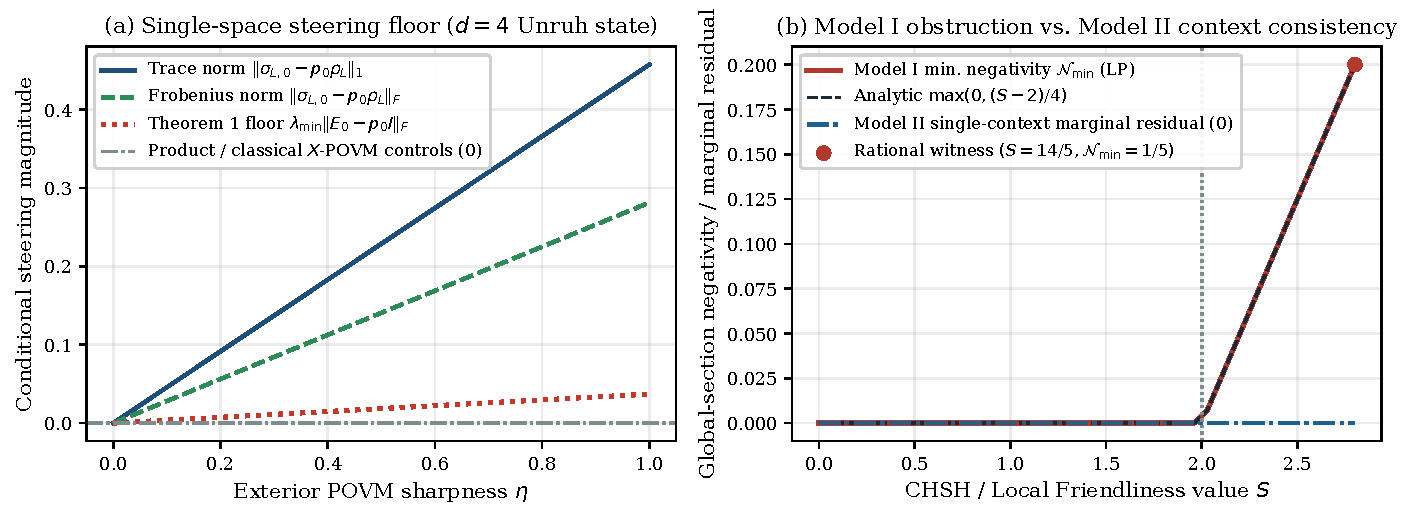
\includegraphics[width=\linewidth]{figures/fig1_steering_and_lf_boundary.pdf}
  \caption{Suites~G1 and~G2 (Theorems~\ref{thm:steering}--\ref{thm:branching}). (a)~Single-space outcome-conditioned state change on a $d=4$ truncated bosonic Unruh state ($r=0.7$, $\lambda_{\min}=0.03149$) across unsharp exterior POVM visibility $\eta\in[0,1]$: trace norm ($0.45723$ at $\eta=1$) dominates Frobenius norm ($0.28116$), which dominates the exact Theorem~\ref{thm:steering} floor ($0.03697$), while product-state and classically-correlated $X$-basis negative controls vanish identically ($0.0$). (b)~Model~I minimum signed global-section negativity $\cN_{\min}$ via linear programming matches $\max(0,(S-2)/4)$ \cite{Oas2014} to $8.33\times 10^{-17}$ across all 41 visibility points, hitting $\cN_{\min}=1/5$ at $S=14/5$ (and $0.20711$ at Tsirelson's $2\sqrt{2}$), while Model~II's single-context marginalization residual stays identically $0.0$ (single-setting marginal check; record agreement and two-path composition are audited separately in G2).}
  \label{fig:steering-lf}
\end{figure}

Figure~\ref{fig:steering-lf} summarizes Suites~G1 and~G2: the Schmidt assemblage identity holds to $1.11\times 10^{-16}$, non-selective completeness to $3.18\times 10^{-17}$, the separable two-qubit isotropic-state control ($v=0.25$, eigenvalues $\frac{3}{16},\frac{7}{16}$) satisfies \eqref{eq:werner-steering} to $1.96\times 10^{-17}$ (with nonzero $X$- and $Z$-basis trace change $0.125$, exact $Z$-basis Frobenius norm $\sqrt{2}/16=0.08839 < \frac{1}{2}\|E-p\1_2\|_F=0.35355$, and trivial-effect change $0.0$), LP negativity matches $\max(0,(S-2)/4)$ to $8.33\times 10^{-17}$, the Bell vs.\ $\frac{1}{4}\1_4$ audit confirms identical local marginals ($1.57\times 10^{-16}$) with $Z$-disagreement $0.0$ vs.\ $0.5$, the Kraus orthogonality norm \eqref{eq:kraus-record-orthog} equals $0.0$ for record-preserving readout vs.\ $1.0$ for bit-flip $K_a=X P_a$, the 4D Wigner's friend dilation confirms premeasurement-isometry Kraus completeness ($0.0$), logical-input orthogonality \eqref{eq:kraus-record-orthog} ($0.0$), and $\operatorname{ran}J$ restriction ($0.0$) vs.\ unrestricted $|01\rangle$ disagreement ($1.0$), with $P(x_S\neq x_F)=0.0$ and interference contrast $1.0 - 0.5 = 0.5$, the two-path diamond gives record-subalgebra pullback difference $0.0$ vs.\ environmental difference $4.0$, and the replacer controls verify both distinct-weight non-uniqueness ($a_1=0.37,a_2=0.81$, gap $0.44$) and same-weight distinct-branch non-uniqueness (Layer~1 difference $0.0$, conditional-state trace distance $0.5$).

%==============================================================================
\section{Finite Clock Analogue, Semifinite Segal Entropy Split, and Gravitational Crossed Products}\label{sec:type2}
%==============================================================================

In continuum quantum field theory, local subregion algebras $\cM_O$ are Type~$\mathrm{III}_1$ factors lacking traces and density operators. Following Takesaki \cite{Takesaki1973}, Witten \cite{Witten2022}, Chandrasekaran--Longo--Penington--Witten (CLPW) \cite{CLPW2023}, Chandrasekaran--Penington--Witten \cite{CPW2023}, Jensen--Sorce--Speranza \cite{JensenSorceSperanza2023}, and De Vuyst--Eccles--H\"ohn--Kirklin \cite{DeVuyst2024,DeVuyst2025}, forming the crossed product by the \emph{modular automorphism group} $\sigma^\omega_t$ of a faithful normal state or faithful normal semifinite weight $\omega$ produces a semifinite Type~$\mathrm{II}_\infty$ continuous core $\cM_O\rtimes_{\sigma^\omega}\bbR$ with a faithful normal semifinite trace $\tau_O$ (note that an arbitrary trivial $\bbR$-action yields $\cM_O\bar{\otimes}L(\bbR)$ and does \emph{not} produce a semifinite core).

To keep algebraic facts strictly separated from semiclassical gravity hypotheses, Theorem~\ref{thm:type2-clock} separates (a)~a finite cyclic $\bbZ_K$ toy analogue (no continuum limit to Type~II is claimed) from (b)~an independent operator-algebraic theorem for \emph{Segal entropy} $S_\tau$ on any semifinite von Neumann algebra $(\cM,\tau)$ (building on Segal \cite{Segal1960}, Araki \cite{Araki1976,Araki1977}, Harada--Kosaki \cite{HaradaKosaki2010}, Pods\k{e}dkowska--Wieczorek \cite{PodsedkowskaWieczorek2017}, and Longo--Witten \cite{LongoWitten2023} via a non-circular positive-pairing regularized proof), while Corollary~\ref{cor:grav-entropy} states explicitly the conditional algebraic identity obtained under semiclassical gravitational generalized entropy hypotheses.

\begin{theorem}[Finite $\bbZ_K$ Toy Analogue and Semifinite Segal-Entropy Branch Split]\label{thm:type2-clock}
\leavevmode
\begin{enumerate}
  \item[(a)] \emph{(Finite $\bbZ_K$ group-averaging toy analogue)} Let $\cH_{\mathrm{sys}}\otimes\cH_C^{(K)}$ carry a cyclic unitary constraint representation $W_t = e^{2\pi i t(H_S+H_C)/K}$ ($t\in\bbZ_K$) for integer-spectrum $H_S$ (dim $d_S$) and $H_C=\mathrm{diag}(0,\dots,K-1)$. The invariant subalgebra $\cA_O^{(K)}:=\{A : W_t A W_t^\dagger = A\ \forall t\in\bbZ_K\}\cong\bigoplus_{r=0}^{K-1} M_{d_S}(\bbC)$ (center dimension $K$, linear dimension $K d_S^2$) is finite-dimensional Type~$\mathrm{I}$, and the group average $\cE_{\mathrm{inv}}(X):=\frac{1}{K}\sum_{t=0}^{K-1}W_t X W_t^\dagger$ is a unital, trace-preserving, idempotent Umegaki bimodule conditional expectation \cite{Umegaki1954}:
  \begin{equation}\label{eq:bimodule}
    \cE_{\mathrm{inv}}(A X B) = A\,\cE_{\mathrm{inv}}(X)\,B \qquad \forall\, A,B\in\cA_O^{(K)}.
  \end{equation}
  Every invariant effect $E\in\cA_O^{(K)}$ satisfies exact Born-weight invariance $\Tr(E\,\cE_{\mathrm{inv}}(\rho))=\Tr(E\rho)$. (This finite-group structure serves solely as a finite-dimensional toy analogue and does not construct a continuum limit to Type~$\mathrm{II}$.)
  \item[(b)] \emph{(Semifinite Segal-entropy branch decomposition with regularized domain proof)} Let $(\cM,\tau)$ be any semifinite von Neumann algebra (Type~$\mathrm{I}$, $\mathrm{II}_1$, or $\mathrm{II}_\infty$) equipped with a faithful normal semifinite trace $\tau$, Segal entropy $S_\tau(\rho):=-\tau(\rho\ln\rho)$ \cite{Segal1960,LongoWitten2023} on the finite-entropy normal-state domain $\cD_{\mathrm{ent}}(\cM,\tau):=\{\rho\in L^1(\cM,\tau)_+ : \tau(\rho)=1,\ \tau(|\rho\ln\rho|)<\infty\}$, and Araki relative entropy $D(\rho\|\sigma)$ \cite{Araki1976,Araki1977}. Let $\{\cI_{O,x}\}_{x=1}^m$ be a normal selective instrument mapping $\rho_O\in\cD_{\mathrm{ent}}(\cM,\tau)$ to conditional states $\rho_{O|x}\in\cD_{\mathrm{ent}}(\cM,\tau)$ with Born weights $p_x=\tau(\cI_{O,x}(\rho_O))>0$ ($\sum_{x=1}^m p_x=1$) and ensemble output $\bar{\rho}_O=\sum_{x=1}^m p_x\rho_{O|x}$. Then $\bar{\rho}_O\in\cD_{\mathrm{ent}}(\cM,\tau)$, and the Layer~1 Segal-entropy change $\Delta S_\tau^{\mathrm{L1}}:=S_\tau(\bar{\rho}_O)-S_\tau(\rho_O)$ and Born-weighted Layer~2 average branch change $\overline{\Delta S}_\tau^{\mathrm{L2}}:=\sum_{x=1}^m p_x[S_\tau(\rho_{O|x})-S_\tau(\rho_O)]$ obey the exact \emph{trace-scale-invariant} identity
  \begin{equation}\label{eq:type2-branch-decomp}
    \Delta S_\tau^{\mathrm{L1}} - \overline{\Delta S}_\tau^{\mathrm{L2}}
    \;=\; \chi_\tau\bigl(\{p_x,\rho_{O|x}\}\bigr)
    \;:=\; \sum_{x=1}^m p_x\,D(\rho_{O|x}\|\bar{\rho}_O)
    \;\in\; \bigl[0, H(\{p_x\})\bigr],
  \end{equation}
  where $H(\{p_x\})=-\sum_{x=1}^m p_x\ln p_x$ (equivalently, $\chi_\tau$ is the classical--quantum mutual information of $\sum_x p_x|x\rangle\langle x|\otimes\rho_{O|x}$ on $\ell^\infty(X)\otimes\cM$). Under any semifinite trace rescaling $\tau'=c\tau$ ($c>0$, $\rho'=c^{-1}\rho$), $S_{\tau'}(\rho')=S_\tau(\rho)+\ln c$ (\cite{LongoWitten2023}, Eq.~(20)), so $\ln c$ cancels identically from $\Delta S_\tau^{\mathrm{L1}}$, $\overline{\Delta S}_\tau^{\mathrm{L2}}$, and $\chi_\tau$. As a gravity-free Type~$\mathrm{II}_1$ saturation witness, on any Type~$\mathrm{II}_1$ factor with normalized trace $\tau(\1)=1$ and projection $P$ with $\tau(P)=\frac{1}{2}$, the L\"uders instrument on input $\1$ yields output average $\1$ and branches $2P, 2(\1-P)$ with $S_\tau(\1)=0$ and $S_\tau(2P)=S_\tau(2(\1-P))=-\ln 2$, attaining $\chi_\tau=\ln 2=H(\{\frac{1}{2},\frac{1}{2}\})$.
\end{enumerate}
\end{theorem}

\begin{proof}
(a)~Unitality, trace preservation, $\bbZ_K$-shift invariance, the bimodule identity \eqref{eq:bimodule}, idempotence, and Born-weight invariance are proved algebraically and formalized in \code{OSTQD\_Layer2/\allowbreak Theorem3\_\allowbreak ClockTypeII.lean} (8 audited declarations, including the scalar regularized logarithm bounds below).
(b)~We establish $\bar{\rho}_O\in\cD_{\mathrm{ent}}(\cM,\tau)$ together with cross-logarithm integrability \emph{before} invoking any trace formula for Araki relative entropy, avoiding circularity and avoiding any noncommutative spectral-projection compression. Set $A_x:=\rho_{O|x}$ and $B:=\bar{\rho}_O=\sum_{x=1}^m p_x A_x$. For $A\in L^1(\cM,\tau)_+$ and Borel $f:[0,\infty)\to[0,\infty]$, interpret the positive trace pairing via spectral truncation as
\begin{equation*}
  \langle A, f(B)\rangle_\tau := \sup_{n\ge 1}\,\tau\bigl(A^{1/2}\min\{f(B),n\1\}A^{1/2}\bigr) \in [0,\infty],
\end{equation*}
writing $\tau(A f(B))$ for this pairing and handling signed logarithms as differences of integrable positive and negative parts $(\ln u)_\pm := \max(0,\pm\ln u)$.
\emph{Step 1 (Positive part of $B\ln B$):} Because $u\mapsto (u\ln u)_+=u(\ln u)_+$ is convex and continuous on $[0,\infty)$ with $0\ln 0=0$, applying semifinite trace Jensen convexity (\cite{HaradaKosaki2010}, Theorem~3.4 and Corollary~3.6) to $\mathrm{diag}(A_1,\dots,A_m)$ with contraction column $(\sqrt{p_1}\1,\dots,\sqrt{p_m}\1)^T$ on $(\cM,\tau)$ yields
\begin{equation*}
  T_+ := \tau\bigl(B(\ln B)_+\bigr)
  \;\le\; \sum_{x=1}^m p_x\,\tau\bigl(A_x(\ln A_x)_+\bigr) < \infty.
\end{equation*}
\emph{Step 2 (Regularized cross-logarithm integrability without projection insertion):} For every $0<\eta\le 1$, spectral functional calculus on $B$ (whose scalar inequalities are machine-checked in \code{regularized\_\allowbreak log\_\allowbreak domination\_\allowbreak bounds}) gives
\begin{equation*}
  0 \;\le\; \bigl(\ln(B+\eta\1)\bigr)_+ \;\le\; \ln(B+\1) \;\le\; (\ln B)_+ + (\ln 2)\1.
\end{equation*}
Since $B\ge p_x A_x$, positive trace pairing yields the $\eta$-uniform positive-part upper bound
\begin{equation*}
  \tau\bigl(A_x(\ln(B+\eta\1))_+\bigr)
  \;\le\; p_x^{-1}\tau\bigl(B\ln(B+\1)\bigr)
  \;\le\; p_x^{-1}\bigl(T_+ + \ln 2\bigr) =: U_x < \infty.
\end{equation*}
Conversely, $B+\eta\1 \ge p_x(A_x+\eta\1) > 0$ (interpreted in positive-operator form order for unbounded $A_x,B$, with operator monotonicity of $\ln$ applied via the integral representation in bounded resolvents $\ln(X+\eta\1)=\int_0^\infty\bigl[(t+1)^{-1}-(X+\eta\1+t\1)^{-1}\bigr]\,dt$) gives $\ln(B+\eta\1)\ge\ln(A_x+\eta\1)+(\ln p_x)\1$. Pairing this inequality \emph{directly with $A_x$} (without inserting any noncommutative projection) yields
\begin{equation*}
  \tau\bigl(A_x\ln(B+\eta\1)\bigr)
  \;\ge\; \tau\bigl(A_x\ln(A_x+\eta\1)\bigr) + \ln p_x
  \;\ge\; \tau(A_x\ln A_x) + \ln p_x =: L_x > -\infty,
\end{equation*}
using $u\ln(u+\eta)\ge u\ln u$ for $u>0$ and $A_x\in\cD_{\mathrm{ent}}(\cM,\tau)$. For every $\eta>0$, $(\ln(B+\eta\1))_-$ is bounded (by $|\ln\eta|$) while the positive part is controlled uniformly by $U_x$, so subtracting yields the $\eta$-uniform negative-part bound
\begin{equation*}
  \tau\bigl(A_x(\ln(B+\eta\1))_-\bigr)
  \;=\; \tau\bigl(A_x(\ln(B+\eta\1))_+\bigr) - \tau\bigl(A_x\ln(B+\eta\1)\bigr)
  \;\le\; U_x - L_x < \infty.
\end{equation*}
Because $B\ge p_x A_x$, $\ker B\subseteq\ker A_x$, so all pairings act on $\supp B$. Letting $\eta\downarrow 0$, monotone convergence applies to $(\ln(B+\eta\1))_-\uparrow (\ln B)_-$ on $\supp B$ and the $\eta$-independent upper bound $(\ln(B+\eta\1))_+\le\ln(B+\1)$ controls the positive part by dominated convergence, establishing $\tau(A_x|\ln B|)<\infty$ for each $x=1,\dots,m$. Summing over the finite ensemble gives
\begin{equation*}
  \tau(B|\ln B|) = \sum_{x=1}^m p_x\,\tau(A_x|\ln B|) < \infty,
\end{equation*}
proving $B\in\cD_{\mathrm{ent}}(\cM,\tau)$ and cross-logarithm integrability prior to applying the relative-entropy trace identity.
\emph{Step 3 (Trace identity and Holevo bounds):} Because $B\ge p_x A_x$, Araki's relative entropy for possibly non-faithful normal states (\cite{Araki1976}; \cite{Araki1977}, Definition~3.1 and Theorem~3.6) satisfies $0\le D(A_x\|B)\le D(A_x\|p_x A_x)=-\ln p_x<\infty$. In the semifinite standard representation $L^2(\cM,\tau)$, the relative modular operator $\Delta_{B,A_x}$ acts on $\supp A_x$ by left multiplication by $B$ and right multiplication by $A_x^{-1}$; since $A_x,B\in\cD_{\mathrm{ent}}(\cM,\tau)$ and Step~2 guarantees $\tau(A_x|\ln B|)<\infty$, evaluating $-\langle A_x^{1/2},\,(\ln\Delta_{B,A_x})A_x^{1/2}\rangle$ yields the semifinite trace formula $D(A_x\|B)=\tau(A_x\ln A_x)-\tau(A_x\ln B)$ (\cite{LongoWitten2023}, \S4--\S5, Eqs.~(19)--(20); \cite{PodsedkowskaWieczorek2017}). Multiplying by $p_x$ and summing gives $\sum_x p_x D(A_x\|B)=S_\tau(B)-\sum_x p_x S_\tau(A_x)=\Delta S_\tau^{\mathrm{L1}}-\overline{\Delta S}_\tau^{\mathrm{L2}}\in[0,H(\{p_x\})]$. Trace-rescaling invariance $S_{c\tau}(c^{-1}\rho)=S_\tau(\rho)+\ln c$ is immediate and its additive cancellation is verified in \code{segal\_\allowbreak entropy\_\allowbreak scale\_\allowbreak invariance}. Direct evaluation gives the Type~$\mathrm{II}_1$ L\"uders saturation witness.
\end{proof}

\begin{corollary}[Conditional Semiclassical Identity for Gravitational Crossed Products]\label{cor:grav-entropy}
Under the hypotheses of Theorem~\ref{thm:type2-clock}(b), let $\cA_O^{\mathrm{cp}}=\cM_O\rtimes_{\sigma^\omega}\bbR$ be a gravitational observer-clock crossed product formed with the modular automorphism group $\sigma^\omega_t$ \cite{Witten2022,JensenSorceSperanza2023}. Following Jensen--Sorce--Speranza (\cite{JensenSorceSperanza2023}, \S\S5.3--5.5), in bounded regions where an observer-energy projection ($q_O\ge 0$, as in a de~Sitter static patch \cite{CLPW2023}) yields a finite-trace projection $P$ with $0<\tau_O(P)<\infty$, the corner $P\cA_O^{\mathrm{cp}}P$ is Type~$\mathrm{II}_1$; by contrast, in asymptotic regions the distinct positive ADM-energy projection has divergent trace, leaving a Type~$\mathrm{II}_\infty$ algebra. Fix the convention that $S_{\mathrm{gen}}(\rho)=\langle A/(4G_N\hbar)\rangle_\rho + S_{\mathrm{matter}}(\rho)$ denotes the bare horizon-area plus matter generalized entropy (excluding clock/ADM energy-distribution entropy), and suppose as an additional semiclassical hypothesis that the input $\rho_O$, every conditional branch $\rho_{O|x}$, and the ensemble output $\bar{\rho}_O$ all lie in a common semiclassical regime where
\begin{equation}\label{eq:semiclassical-corr}
  S_\tau(\rho) = S_{\mathrm{gen}}(\rho) + C + \delta(\rho),
\end{equation}
with state-independent renormalization constant $C$ and state-dependent correction $\delta(\rho)$ collecting clock/ADM energy-distribution entropy, clock--field entanglement, and subleading semiclassical terms (\cite{JensenSorceSperanza2023}, Eqs.~(5.32), (5.52)--(5.53); \cite{DeVuyst2025}, \S6). Then $C$ cancels identically across \eqref{eq:type2-branch-decomp}, yielding the conditional algebraic identity
\begin{equation}\label{eq:grav-branch-split}
  \Delta S_{\mathrm{gen}}^{\mathrm{L1}} - \overline{\Delta S}_{\mathrm{gen}}^{\mathrm{L2}}
  \;=\; \chi_\tau\bigl(\{p_x,\rho_{O|x}\}\bigr) - \delta(\bar{\rho}_O) + \sum_{x=1}^m p_x\,\delta(\rho_{O|x}).
\end{equation}
In particular, if an independent semiclassical bound $|\delta(\rho)|\le\eta_{\mathrm{sc}}$ holds uniformly on $\bar{\rho}_O$ and every branch $\rho_{O|x}$, then $\Delta S_{\mathrm{gen}}^{\mathrm{L1}}-\overline{\Delta S}_{\mathrm{gen}}^{\mathrm{L2}}\in[-2\eta_{\mathrm{sc}},\,H(\{p_x\})+2\eta_{\mathrm{sc}}]$; constructing a concrete gravitational instrument and semiclassical state family that preserves the crossed-product corner and certifies such an $\eta_{\mathrm{sc}}$ bound remains an open problem.
\end{corollary}

\begin{remark}[Conditional GSL Scope and Ozawa Negative Control]\label{rem:ozawa}
(i)~In gravitational crossed products, the Layer~1 generalized second law ($\Delta S_\tau^{\mathrm{L1}}\ge 0$ \cite{CPW2023}) is a statement about \emph{horizon-cut restriction / nested subregion inclusion}, not about arbitrary CPTP instruments (for example, a replacer sending $\frac{1}{2}\1_2$ to $|0\rangle\langle 0|$ gives $\Delta S_\tau^{\mathrm{L1}}=-\ln 2<0$). Whenever $\Delta S_\tau^{\mathrm{L1}}\ge 0$ does hold, Theorem~\ref{thm:type2-clock}(b) implies the \emph{branch-averaged} lower bound $\overline{\Delta S}_\tau^{\mathrm{L2}}\ge\Delta S_\tau^{\mathrm{L1}}-H(\{p_x\})$ (distinct from branch-by-branch monotonicity), and under Corollary~\ref{cor:grav-entropy} the corresponding $S_{\mathrm{gen}}$ bound acquires the explicit term $\delta(\bar{\rho}_O)-\sum_x p_x\delta(\rho_{O|x})$.
(ii)~As proved by Ozawa \cite{Ozawa1986} resolving Groenewold's conjecture \cite{Groenewold1971}, the information gain $I_{\mathrm{GO}}:=-\overline{\Delta S}_\tau^{\mathrm{L2}}$ can be strictly negative for general CP instruments: a noisy measure-and-prepare instrument $\cI_x(\rho)=\Tr(E_x\rho)[(1-q)|x\rangle\langle x|+q\frac{\1}{2}]$ yields in general $\chi_\tau=h_2\bigl((1-q)p_1+\frac{q}{2}\bigr)-h_2(q/2)$ (vanishing at $q=1$ for all $p_1$ since both branches output $\frac{1}{2}\1$, and giving $h_2(0.3)-h_2(\frac{1}{4})\approx 0.04853$ at $p_1=0.1, q=\frac{1}{2}$). Under equal Born weights $p_0=p_1=\frac{1}{2}$ (attained by $E_x=|x\rangle\langle x|$ on pure input $|+\rangle\langle +|$), $I_{\mathrm{GO}}=-h_2(q/2)<0$ for every $q\in(0,1]$ (reaching $-\ln 2\approx -0.69315$ at $q=1$), while $\chi_\tau=\ln 2 - h_2(q/2)\in[0,\ln 2]$ remains strictly non-negative.
\end{remark}

\begin{figure}[!tb]
  \centering
  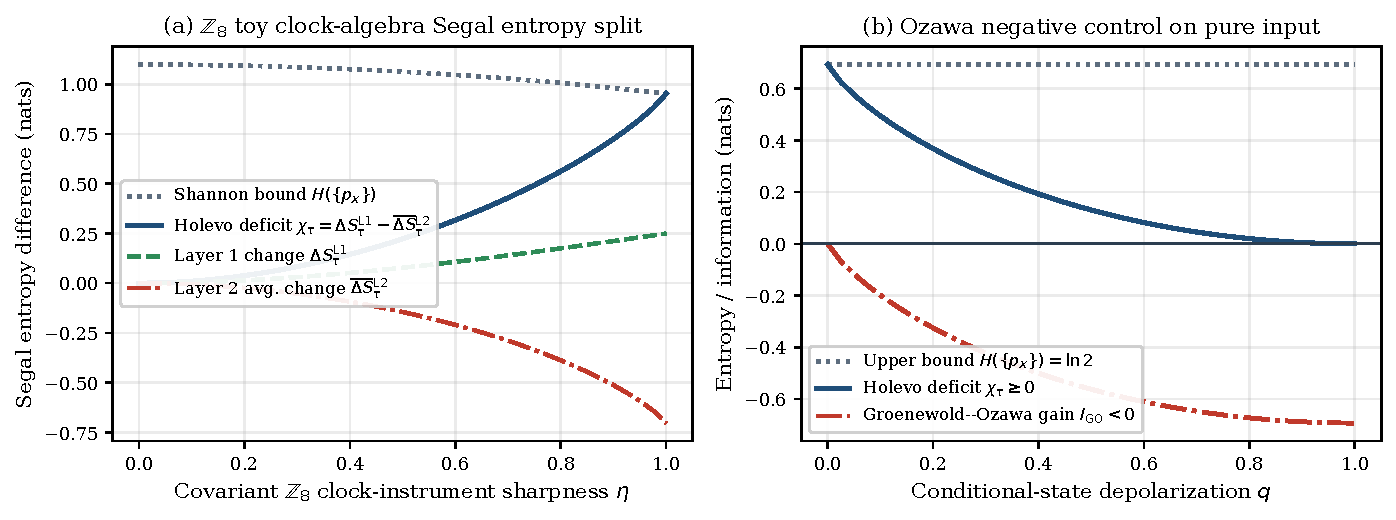
\includegraphics[width=\linewidth]{figures/fig2_type2_clock_entropy.pdf}
  \caption{Suite~G3 (Theorem~\ref{thm:type2-clock} and Corollary~\ref{cor:grav-entropy}). (a)~$\bbZ_8$ finite-group toy clock algebra ($\cA_O^{(8)}\cong\bigoplus_{r=0}^7 M_3(\bbC)$, linear dim $72$) across covariant instrument sharpness $\eta\in[0,1]$: $\Delta S_\tau^{\mathrm{L1}}=+0.24903$ and $\overline{\Delta S}_\tau^{\mathrm{L2}}=-0.70330$ at $\eta=1$, matching $\chi_\tau=0.95232=H(\{p_x\})$ to $8.92\times 10^{-16}$ and invariant under trace rescalings $c\in\{0.1,1,10,100\}$ to $4.00\times 10^{-15}$. (b)~Ozawa (1986) negative control on pure input $|+\rangle\langle +|$ with $E_x=|x\rangle\langle x|$ ($p_0=p_1=\frac{1}{2}$): $I_{\mathrm{GO}}<0$ ($-0.56234$ at $q=0.5$, $-\ln 2=-0.69315$ at $q=1$) while $\chi_\tau\in[0,\ln 2]$ holds universally.}
  \label{fig:type2-clock}
\end{figure}

Figure~\ref{fig:type2-clock} confirms Suite~G3: the $\bbZ_8$ Umegaki conditional expectation obeys idempotence to $1.29\times 10^{-14}$, bimodule equivariance to $1.53\times 10^{-13}$, trace preservation to $9.93\times 10^{-16}$, and dressed-operator invariance to $1.71\times 10^{-15}$ (vs.\ undressed commutator $5.65685$); across $K\in\{4,8,16,32\}$, the invariant projection weight matches $\Tr(\Pi_0\rho_S^{\mathrm{th}})=1/(1+e^{-0.8}+e^{-1.6})=0.605611$ to $1.11\times 10^{-16}$ (testing finite-group averaging invariance, not a continuum Type~II limit); as a finite-matrix substitution and constant-cancellation check of Corollary~\ref{cor:grav-entropy} (whose magnitude and sign depend on the toy ansatz rather than semiclassical gravity), assembling $S_{\mathrm{gen}}$ from \eqref{eq:semiclassical-corr} with $\delta(\rho)=0.1\,I(S:C)_\rho$ confirms \eqref{eq:grav-branch-split} to $3.33\times 10^{-16}$ with non-vanishing state-dependent term $-\delta(\bar{\rho}_O)+\sum_x p_x\delta(\rho_{O|x})=+0.003909\neq 0$; a normalized-trace ($\tau=\frac{1}{2}\Tr$) L\"uders projection check confirms exact saturation $\chi_\tau=\ln 2$ (err $0.0$) and an unequal-weight Ozawa check ($p_1=0.1$) confirms $\chi_\tau=0.04853$ at $q=0.5$ (err $1.11\times 10^{-16}$) and $0.0$ at $q=1$; and a noncommutative rescaled-trace check ($\tau=\frac{1}{2}\Tr$ on $M_2(\bbC)$, $p=(\frac{1}{4},\frac{3}{4})$, $\rho_1=\mathrm{diag}(1.999,0.001)$, $\bar{\rho}=[[1,-\frac{1}{2}],[-\frac{1}{2},1]]$, $\eta=10^{-6}$) directly validates the positive-pairing bounds of Step~2 ($0.20273\le U_1=3.98898$, $0.33789\le U_2=1.32966$, negative pairings $0.34657\le U_1-L_1=4.68643$, $0.11552\le U_2-L_2=1.30560$, cross-logarithm sum error $5.55\times 10^{-17}$, and $\chi_\tau=0.27520\le H=0.56234$).

%==============================================================================
\section{Sharp Polar-Isometric Pullback Bounds and Sequential Evaporation vs.\ Postselected Dictionaries}\label{sec:nonisometric}
%==============================================================================

We now analyze how fundamental selective measurements pull back across a finite-dimensional non-isometric holographic encoding $V_u$ \cite{Akers2024} (noting that our operator-norm code subspace $\cC$ is distinct from Akers et al.'s sub-exponential complexity state set \cite{Akers2024}, \S\S2,\,3.6, and distinguishing the interior dictionary $V_n:\cH_C\otimes\cH_{L_n}\to\cH_{\mathrm{BH}(n)}$ of output dimension $d_{\mathrm{BH}}(n)$ from its Bell-code restriction $\tilde{V}_n:\cH_C\to\cH_{\mathrm{fund}}$ of output dimension $d_{\mathrm{fund}}$). Combining the classical positive-operator angle bound of Kantorovich \cite{Kantorovich1948} and Gustafson \cite{Gustafson1968} with the sharp unnormalized polar bound, mixed-state purification contraction, and Helstrom-POVM saturation witnesses, we also separate a strictly causal sequential unitary evaporation circuit $W_n^{\mathrm{seq}}$ from time-indexed postselected dictionary benchmarks $(V_n,W_{\mathrm{pol},n})$.

\begin{theorem}[Sharp Polar-Isometric Pullback Bounds and Causal Sequential Evaporation vs.\ Postselected Benchmarks]\label{thm:nonisometric}
Let $V:\cH_{\mathrm{eff}}\to\cH_{\mathrm{fund}}$ be a linear map, $\{E_{B,x}\}_{x\in X}$ any fundamental POVM on $\cH_{\mathrm{fund}}$ ($\sum_x E_{B,x}=\1_{\mathrm{fund}}$), $\tilde{E}_{A,x}:=V^\dagger E_{B,x} V\ge 0$, and unnormalized pullback weights $p_{B,x}(\rho_A):=\Tr(E_{B,x}V\rho_A V^\dagger)=\Tr(\tilde{E}_{A,x}\rho_A)$ for $\rho_A\in\cD(\cH_{\mathrm{eff}})$.
\begin{enumerate}
  \item[(a)] \emph{(Exact pullback sum, kernel annihilation, and sign of $\Delta_{\mathrm{norm}}$)} $\sum_x\tilde{E}_{A,x}=V^\dagger V$, so that $\sum_x p_{B,x}(\rho_A)=1-\Delta_{\mathrm{norm}}(\rho_A)$, where $\Delta_{\mathrm{norm}}(\rho_A):=\Tr\bigl((\1_{\mathrm{eff}}-V^\dagger V)\rho_A\bigr)$. Note that $p_{B,x}$ are unnormalized weights (distinct from normalized probabilities and postselection success probabilities), and $\Delta_{\mathrm{norm}}(\rho_A)$ can be negative whenever $V^\dagger V$ has eigenvalues exceeding $1$. Whenever $d_{\mathrm{eff}}>d_{\mathrm{fund}}$, $\ker V\neq\{0\}$, and every state $|v\rangle\langle v|$ with $v\in\ker V$ suffers total annihilation: $p_{B,x}=0$ for all $x$ and $\Delta_{\mathrm{norm}}=1$.
  \item[(b)] \emph{(Uniformly sharp polar-isometric $\ell^1$ bounds on a code subspace $\cC$)} Suppose $\cC\subseteq\cH_{\mathrm{eff}}$ (orthogonal projector $P_\cC$, $\dim\cC\ge 2$) is an $\varepsilon$-approximate isometry subspace:
  \begin{equation}\label{eq:approx-iso}
    \normOp{P_\cC(V^\dagger V - \1_{\mathrm{eff}})P_\cC} \le \varepsilon < 1,
    \qquad
    a := \sqrt{1-\varepsilon},\quad b := \sqrt{1+\varepsilon}.
  \end{equation}
  Let $V P_\cC = W M$ be the polar decomposition with exact isometry $W:\cC\to\cH_{\mathrm{fund}}$ ($W^\dagger W=P_\cC$) and $M=(P_\cC V^\dagger V P_\cC)^{1/2}$ ($a P_\cC \le M \le b P_\cC$), and let $p_{A,x}^{\mathrm{pol}}(\rho_A):=\Tr(E_{B,x}W\rho_A W^\dagger)$ be the exact polar-isometric probabilities. Using the $\ell^1$ convention $\sum_x|p_x-q_x|$ (equal to $2 D_{\mathrm{TV}}(p,q)$ for normalized distributions), for \emph{every} density operator $\rho_A$ supported on $\cC$ and \emph{every} fundamental POVM $\{E_{B,x}\}$,
  \begin{equation}\label{eq:polar-sharp-unnorm}
    \sum_{x\in X}\bigl|p_{B,x}(\rho_A) - p_{A,x}^{\mathrm{pol}}(\rho_A)\bigr|
    \;\le\; \normTr{V\rho_A V^\dagger - W\rho_A W^\dagger}
    \;\le\; b - a \;=\; \sqrt{1+\varepsilon} - \sqrt{1-\varepsilon},
  \end{equation}
  and, setting $Z:=\Tr(V\rho_A V^\dagger)=\Tr(M^2\rho_A)\in[1-\varepsilon,1+\varepsilon]$ and $\hat{p}_{B,x}(\rho_A):=p_{B,x}(\rho_A)/Z$,
  \begin{equation}\label{eq:polar-sharp-norm}
    \sum_{x\in X}\bigl|\hat{p}_{B,x}(\rho_A) - p_{A,x}^{\mathrm{pol}}(\rho_A)\bigr|
    \;\le\; \left\|\frac{V\rho_A V^\dagger}{Z} - W\rho_A W^\dagger\right\|_1
    \;\le\; \frac{2(b-a)}{b+a} \;=\; \frac{2\varepsilon}{1+\sqrt{1-\varepsilon^2}}.
  \end{equation}
  On pure states, the normalized bound \eqref{eq:polar-sharp-norm} rests on the classical Kantorovich--Gustafson positive-operator angle / antieigenvalue inequalities $\inf_{\|\psi\|=1}\langle\psi,M\psi\rangle/\|M\psi\|\ge 2\sqrt{ab}/(a+b)$ and $\sup_{\|\psi\|=1}\sin\angle(\psi,M\psi)\le (b-a)/(b+a)$ for spectral envelope bounds $0<a\1\le M\le b\1$, with equality when $a$ and $b$ are the actual extremal eigenvalues of $M$ \cite{Kantorovich1948,Gustafson1968}. Both constants in \eqref{eq:polar-sharp-unnorm}--\eqref{eq:polar-sharp-norm} are \emph{uniformly sharp} over pairs $(M,\rho_A)$ satisfying $a\1\le M\le b\1$: for $M=\mathrm{diag}(a,b)$, \eqref{eq:polar-sharp-unnorm} is saturated by $|\psi_u\rangle=\frac{1}{\sqrt{2}}(|a\rangle+|b\rangle)$ and \eqref{eq:polar-sharp-norm} is saturated by $|\psi_n\rangle=\sqrt{\frac{b}{a+b}}|a\rangle+\sqrt{\frac{a}{a+b}}|b\rangle$, with the optimal two-outcome Helstrom POVM attaining equality on the left-hand $\ell^1$ sums as well. Operationally, \eqref{eq:polar-sharp-norm} describes a \emph{success-conditioned} distribution: applying the individually normalized map $\rho\mapsto M\rho M/\Tr(M^2\rho)$ branch-by-branch with equal weights to $Z$- vs.\ $X$-decompositions of $\frac{1}{2}\1_2$ at $M=\mathrm{diag}(a,b)$ produces a Gisin-type ensemble trace distance $\varepsilon/2$ (and $\Delta\langle Z\rangle=\varepsilon$), whereas embedding $V$ as a contractive success Kraus operator $K:=V/\normOp{V}$ with success-probability reweighting $p_i\Tr(K\rho_i K^\dagger)$ restores exact ensemble linearity alongside the complementary failure branch.
  \item[(c)] \emph{(Causal sequential unitary evaporation circuit vs.\ time-indexed postselected benchmarks)} Take $N_{\mathrm{BH},0}$ initial black hole qubits ($d_{\mathrm{fund}}=2^{N_{\mathrm{BH},0}}$, $d_{\mathrm{BH}}(n)=2^{N_{\mathrm{BH},0}-n}$, $d_{\mathrm{rad}}(n)=2^n$, $n=0,\dots,N_{\mathrm{BH},0}$).
  \begin{enumerate}
    \item[(c.1)] \emph{Strictly causal sequential unitary circuit $W_n^{\mathrm{seq}}$:} Starting from an initial isometric diary encoding $W_0^{\mathrm{seq}}:\cH_C\to\cH_{B_0}$, apply at each step $n\ge 1$ an isometric emission step $U_n:\cH_{B_{n-1}}\to\cH_{B_n}\otimes\cH_{R_{\mathrm{new},n}}$ acting solely on the remaining black hole, followed by the canonical tensor permutation $\Pi_n:\cH_{B_n}\otimes\cH_{R_{\mathrm{new},n}}\otimes\cH_{R_{n-1}}\to\cH_{B_n}\otimes\cH_{R_{n-1}}\otimes\cH_{R_{\mathrm{new},n}}$ appending $R_{\mathrm{new},n}$ to the right of $R_{n-1}$:
    \begin{equation}\label{eq:seq-circuit}
      W_n^{\mathrm{seq}} = \Pi_n\bigl(U_n \otimes \1_{R_{n-1}}\bigr) W_{n-1}^{\mathrm{seq}}.
    \end{equation}
    Then for \emph{every} choice of isometries $\{U_n\}$, \emph{every} input $\rho_C$, and every $n\ge 1$, the emitted radiation marginal obeys exact sequential compatibility:
    \begin{equation}\label{eq:seq-compat}
      \Tr_{R_{\mathrm{new},n}}\!\bigl(\rho_{R_n}\bigr) = \rho_{R_{n-1}},
      \qquad
      \rho_{R_n} := \Tr_{B_n}\!\bigl(W_n^{\mathrm{seq}}\rho_C (W_n^{\mathrm{seq}})^\dagger\bigr),
    \end{equation}
    and at every step $n$ the remaining-black-hole entanglement fidelity on the maximally mixed code input obeys the universal intermediate dimension bottleneck $F_{\mathrm{rem}}(n)\le\min(1,\,d_{\mathrm{BH}}(n)^2/d_C^2)$ across all CPTP decoders (\cite{Soga2026OSTQD}, Theorem~5), with exact endpoint identities at $d_{\mathrm{BH}}=1$: perfect radiation recovery is attainable and achieved on the maximally mixed code input by the Petz recovery map ($F_{\mathrm{rad}}(N_{\mathrm{BH},0})=1$), while remaining-black-hole fidelity drops to $F_{\mathrm{rem}}(N_{\mathrm{BH},0})=1/d_C^2$ (Figure~\ref{fig:nonisometric} evaluates both curves using the Petz recovery map on the maximally mixed code input). By contrast, a non-monotonic Page-like radiation entropy curve is \emph{circuit-dependent} rather than forced by \eqref{eq:seq-compat}: an identity circuit ($U_n=\1$) on product encoding $|+\rangle\otimes|0\rangle^{\otimes(N_{\mathrm{BH},0}-1)}$ yields $S(R_n)=0$ for all $n$, whereas Haar-scrambling steps $\{U_n\}$ generate a Page-like hump (Suite~G4).
    \item[(c.2)] \emph{Separate time-indexed postselected non-isometric dictionary family $(V_n,W_{\mathrm{pol},n})$:} Let $\iota_n:\cH_C\to\cH_C\otimes\cH_{L_n}\otimes\cH_{R_n}$ be $\iota_n|\psi\rangle=|\psi\rangle_C\otimes|\mathrm{Bell}\rangle_{L_n R_n}^{\otimes n}$. Whenever the rank-obstruction threshold $m_n:=d_C 2^n > r_n:=d_{\mathrm{BH}}(n) \iff 2n > N_{\mathrm{BH},0}-\log_2 d_C$ holds, define for \emph{arbitrary} $d_C$ (not restricted to powers of $2$) the scaled co-isometric interior dictionary $V_n:\cH_C\otimes\cH_{L_n}\to\cH_{\mathrm{BH}(n)}$ by $V_n:=\sqrt{m_n/r_n}\,P_{r_n} U_{\mathrm{scr},n}$, where $P_{r_n}:\bbC^{m_n}\to\bbC^{r_n}$ projects onto the first $r_n$ coordinates and $U_{\mathrm{scr},n}\in U(m_n)$ (reducing to the tensor-factor postselection $\sqrt{d_{P_n}}(\langle 0|_{P_n}\otimes\1_{\mathrm{BH}(n)})U_{\mathrm{scr},n}$ whenever $r_n\mid m_n$, e.g.\ when $d_C$ is a power of $2$, cf.\ \cite{Akers2024}, \S2.1 with auxiliary input $|\psi_0\rangle_f$). This yields the code restriction $\tilde{V}_n:=(V_n\otimes\1_{R_n})\iota_n:\cH_C\to\cH_{\mathrm{fund}}$ obeying $\mathbb{E}[V_n^\dagger V_n]=\1_{m_n}$ and $\mathbb{E}[\tilde{V}_n^\dagger\tilde{V}_n]=\1_C$ under Haar $U_{\mathrm{scr},n}$ for all $m_n>r_n$ (with high-probability approximate isometry requiring separate Haar measure concentration \cite{Akers2024}). On every full-column-rank realization (automatically satisfied whenever \eqref{eq:approx-iso} holds with $\varepsilon_n<1$), the canonical polar factor defines a unique polar isometry $W_{\mathrm{pol},n}:\cH_C\to\cH_{\mathrm{fund}}$, whereas individual realizations can violate $\varepsilon_n<1$ or full column rank (e.g.\ $N_{\mathrm{BH},0}=2, d_C=4, n=2, U_{\mathrm{scr}}=\1_{16}$ gives $\tilde{V}^\dagger\tilde{V}=\mathrm{diag}(4,0,0,0)$ and $\varepsilon=3>1$, where the polar factor is only a partial isometry with non-unique isometric extensions onto $\ker\tilde{V}$). Each snapshot satisfies \eqref{eq:polar-sharp-unnorm}--\eqref{eq:polar-sharp-norm} whenever $\tilde{V}_n$ satisfies \eqref{eq:approx-iso} with $\varepsilon_n<1$. Regarding sequential compatibility \eqref{eq:seq-compat}:
    \emph{(i)~Stinespring characterization:} two full-column-rank polar isometries $W_{\mathrm{pol},n-1},W_{\mathrm{pol},n}$ define trace-preserving radiation channels and satisfy \eqref{eq:seq-compat} for all inputs (equivalently on all $d_C^2$ matrix units) if and only if both are Stinespring dilations of the same prior-radiation channel with equal environment dimension $d_{\mathrm{BH}}(n-1)=2d_{\mathrm{BH}}(n)$, hence are linked by an environment unitary $U_n:\cH_{B_{n-1}}\to\cH_{B_n}\otimes\cH_{R_{\mathrm{new},n}}$ via \eqref{eq:seq-circuit} (\cite{Watrous2018}, Corollary~2.24; no minimality assumption is needed because the environment dimensions coincide).
    \emph{(ii)~Kernel activation alone does not force incompatibility:} at $n=1$, $\dim\cH_{R_0}=1$ makes $\Tr_{R_1}\rho_{R_1}=1=\rho_{R_0}$ automatic for every full-column-rank realization (e.g.\ $N_{\mathrm{BH},0}=1,d_C=2,V_1=\sqrt{2}(1,0,0,1)\implies\tilde{V}_1=\1_2$); even with nontrivial prior radiation, at $N_{\mathrm{BH},0}=2,d_C=2$, the scaled co-isometries $V_1=\sqrt{2}(|0\rangle_{B_1}\langle 0,0|_{CL_1}+|1\rangle_{B_1}\langle 1,0|_{CL_1})$ and $V_2=2(\langle 0,(0,0)|_{CL_2}+\langle 1,(0,1)|_{CL_2})$ both possess nontrivial kernels ($\dim\ker V_1=2$, $\dim\ker V_2=7$) yet yield exact isometries $\tilde{V}_1|i\rangle=|i\rangle_{B_1}|0\rangle_{R_1}$ and $\tilde{V}_2|i\rangle=|0\rangle_{R_1}|i\rangle_{R_{\mathrm{new}}}$ obeying \eqref{eq:seq-compat} identically across all four matrix units.
    \emph{(iii)~Explicit incompatibility benchmark and causal conditioning caveat:} by contrast, in Suite~G4's fixed-seed independent-Haar realization ($N_{\mathrm{BH},0}=6,d_C=2$), $W_{\mathrm{pol},n}$ (on $\frac{1}{2}\1_2$, on pure input $|0\rangle\langle 0|$, and across the full $d_C^2=4$ Choi basis) violates \eqref{eq:seq-compat} for $n=3,\dots,6$ (above the rank-obstruction threshold $2n>5$, distinct from a thermodynamic Page time), certifying by~(i) that this isometric sequence cannot arise from any sequential circuit \eqref{eq:seq-circuit}. For the renormalized raw dictionary outputs $\tilde{V}_n\rho_C\tilde{V}_n^\dagger/Z_n$, the discrepancy against \eqref{eq:seq-compat} measures specifically the mismatch of \emph{individually success-conditioned snapshot outputs}: even in a strictly causal device, conditioning on a later outcome updates prior radiation (e.g.\ measuring $Z$ on half of a Bell pair and conditioning on $0$ updates the partner from $\frac{1}{2}\1_2$ to $|0\rangle\langle 0|$, trace distance $\frac{1}{2}$, whereas averaging over outcomes restores $\frac{1}{2}\1_2$); diagnosing physical backward signaling requires a full sequential instrument with unnormalized outcome states $\sigma^{(n,s)}$ satisfying $\sum_s\Tr_{R_{\mathrm{new}}}\sigma^{(n,s)}=\rho_{R_{\mathrm{old}}}^{(n-1)}$ (\cite{Chiribella2009}, Theorem~5, Eq.~(40)). Moreover, because $\tilde{V}_n^\dagger\tilde{V}_n = 2^{-n}\Tr_{L_n}(V_n^\dagger V_n)$, the maximally mixed trace obeys $Z_n(\frac{1}{d_C}\1_{d_C})=\Tr(V_n^\dagger V_n)/(d_C 2^n)=1$ identically for every realization, whereas on pure input $|0\rangle\langle 0|$ at $n=5,6$ ($Z_5\neq 1\neq Z_6$) renormalization acts nontrivially while preserving a large sequential discrepancy (Suite~G4).
  \end{enumerate}
\end{enumerate}
\end{theorem}

\begin{proof}
(a)~Immediate from linearity, cyclicity of trace, and $V v = 0\implies V|v\rangle\langle v|V^\dagger=0$.
(b)~Because $W$ is an isometry, $\normTr{V\rho_A V^\dagger - W\rho_A W^\dagger}=\normTr{M\rho_A M - \rho_A}$ and similarly for the normalized state. First consider a pure state $\rho_A=|\psi\rangle\langle\psi|$, setting $s:=\langle\psi|M|\psi\rangle>0$, $Z:=\langle\psi|M^2|\psi\rangle>0$, $c:=a+b$, and $k:=ab=\sqrt{1-\varepsilon^2}$. Since $a\1\le M\le b\1$ implies $(b\1-M)(M-a\1)\ge 0$, we have $M^2\le c M - k\1$, hence $Z\le c s - k$, while $a^2+b^2=2$ gives $c^2=2+2k$ and $(b-a)^2=2-2k$. Since $\Delta:=M|\psi\rangle\langle\psi|M-|\psi\rangle\langle\psi|$ has rank at most $2$, its two candidate eigenvalues (allowing zero when $M|\psi\rangle\parallel|\psi\rangle$) satisfy $\lambda_1+\lambda_2=Z-1$ and $\lambda_1\lambda_2 = s^2 - Z$, giving
\begin{equation*}
  \normTr{M|\psi\rangle\langle\psi|M - |\psi\rangle\langle\psi|}^2
  = (\lambda_1-\lambda_2)^2 = (Z+1)^2 - 4 s^2.
\end{equation*}
Using $0\le Z\le c s - k$ and $c^2=2+2k$ yields
\begin{equation*}
  (Z+1)^2 - 4 s^2 \;\le\; (c s - k + 1)^2 - 4 s^2
  = (b-a)^2 - (b-a)^2\Bigl(s-\frac{c}{2}\Bigr)^2 \;\le\; (b-a)^2,
\end{equation*}
proving \eqref{eq:polar-sharp-unnorm} on pure states, with equality at $M=\mathrm{diag}(a,b)$ and $|\psi_u\rangle=(|a\rangle+|b\rangle)/\sqrt{2}$ (where $s=c/2$ and $Z=(a^2+b^2)/2=1$). For the normalized pure state, $\normTr{\frac{M|\psi\rangle\langle\psi|M}{Z}-|\psi\rangle\langle\psi|}=2\sqrt{1-s^2/Z}$, and
\begin{equation*}
  \frac{s^2}{Z} \;\ge\; \frac{s^2}{c s - k} \;\ge\; \frac{4k}{c^2} = \frac{4ab}{(a+b)^2}
  \quad\Longleftrightarrow\quad
  (c s - 2k)^2 \ge 0,
\end{equation*}
yielding $2\sqrt{1-s^2/Z}\le 2\sqrt{1-\frac{4ab}{(a+b)^2}}=\frac{2(b-a)}{b+a}=\frac{2(b^2-a^2)}{(b+a)^2}=\frac{2\varepsilon}{1+\sqrt{1-\varepsilon^2}}$, saturated at $p_a=b/(a+b)$, $p_b=a/(a+b)$ (where $s=2ab/(a+b)$ and $Z=ab$). For a general mixed state $\rho_A$ on $\cC$, purify $\rho_A=\Tr_E|\Psi\rangle\langle\Psi|$ on $\cC\otimes\cH_E$ and apply $M\otimes\1_E$ (which shares the same spectral bounds $[a,b]$ and preserves $Z$); monotonicity of trace norm under $\Tr_E$ yields \eqref{eq:polar-sharp-unnorm}--\eqref{eq:polar-sharp-norm} for all mixed $\rho_A$. Finally, $\sum_x|\Tr(E_{B,x}\Delta)|\le\normTr{\Delta}$ holds for every POVM, with equality for the eigenbasis projectors of $\Delta$; direct evaluation on $Z$- vs.\ $X$-decompositions of $\frac{1}{2}\1_2$ yields the un-reweighted Gisin gap $\varepsilon/2$ vs.\ zero bias under contractive Kraus reweighting.
(c.1)~Because $U_n^\dagger U_n=\1_{B_{n-1}}$, $\Tr_{B_n,R_{\mathrm{new},n}}[\Pi_n(U_n\otimes\1_{R_{n-1}})\rho_{B_{n-1}R_{n-1}}(U_n^\dagger\otimes\1_{R_{n-1}})\Pi_n^\dagger] = \Tr_{B_{n-1}}(\rho_{B_{n-1}R_{n-1}})$ identically.
(c.2)~By unitary invariance of Haar measure on $U(m_n)$, $\mathbb{E}[U_{\mathrm{scr},n}^\dagger P_{r_n}^\dagger P_{r_n} U_{\mathrm{scr},n}] = \frac{r_n}{m_n}\1_{m_n}$, giving $\mathbb{E}[V_n^\dagger V_n]=\1_{m_n}$ and $\mathbb{E}[\tilde{V}_n^\dagger\tilde{V}_n]=\iota_n^\dagger\iota_n=\1_C$. The Stinespring characterization follows from unitary equivalence of Stinespring dilations with equal environment dimension $d_{\mathrm{BH}}(n-1)=2d_{\mathrm{BH}}(n)$. Direct evaluation verifies the $N_{\mathrm{BH},0}=2,d_C=2$ witness $(V_1,V_2)$. Parts~(a), the pure-state real scalar cores and saturation witnesses of (b), the normalized-filter Gisin bias witness (\code{postselected\_\allowbreak normalized\_\allowbreak gisin\_\allowbreak bias\_\allowbreak witness}), general sequential compatibility (c.1), and the compatible non-isometric witness (\code{nonisometric\_\allowbreak kernel\_\allowbreak compatible\_\allowbreak two\_\allowbreak step\_\allowbreak witness}) are machine-checked in \code{OSTQD\_Layer2/\allowbreak Theorem4\_\allowbreak NonIsometricPullback.lean} (10 audited declarations).
\end{proof}

\begin{remark}[Scope Caveat and Dynamical Non-Isometric Circuit Comparison]\label{rem:u4-caveat}
Separating $W_n^{\mathrm{seq}}$ from $(V_n,W_{\mathrm{pol},n})$ clarifies three distinct regimes in dynamical black hole encoding: (1)~\emph{finite-circuit dynamical dictionaries}, such as DeWolfe--Higginbotham \cite{DeWolfeHigginbotham2023} (\S3, Eqs.~(3.3)--(3.4)), which compose backward effective evolution with forward fundamental circuit evolution to enforce dynamical consistency with postselected encodings on dynamically prepared black hole states; (2)~\emph{our all-input Stinespring criterion} (Theorem~\ref{thm:nonisometric}(c)), which characterizes when independently specified polar isometries $W_{\mathrm{pol},n}$ yield identical prior-radiation channels across all code inputs, while separating strictly causal circuits $W_n^{\mathrm{seq}}$ (where at $d_{\mathrm{BH}}=1$, $F_{\mathrm{rad}}(N_{\mathrm{BH},0})=1$ reflects exact recoverability of any isometry into $\cH_{\mathrm{rad}}$, achieved here by the Petz map, rather than a dynamical gravity prediction) from snapshot postselected benchmarks; and (3)~\emph{microscopic autonomous gravitational or $U(N)$ matrix Hamiltonians} that simultaneously obey \eqref{eq:seq-compat} and generate complexity-protected non-isometric interior encodings, which remains an open problem.
\end{remark}

\begin{figure}[!tb]
  \centering
  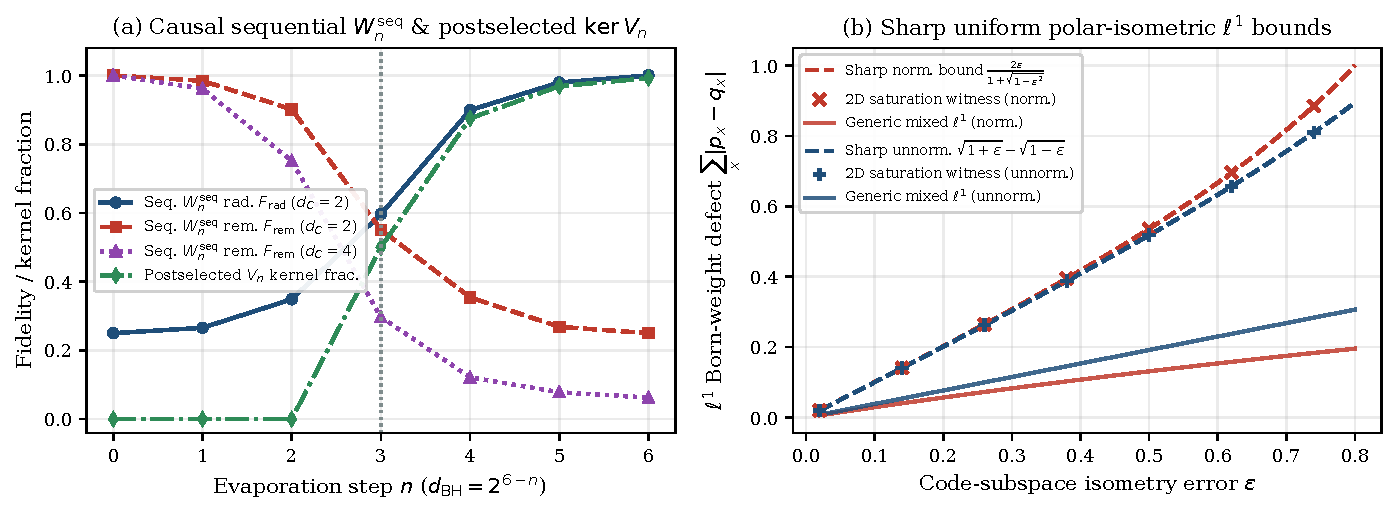
\includegraphics[width=\linewidth]{figures/fig3_dynamical_nonisometric_pullback.pdf}
  \caption{Suite~G4 (Theorem~\ref{thm:nonisometric}). (a)~Strictly causal sequential unitary evaporation circuit $W_n^{\mathrm{seq}}$ ($N_{\mathrm{BH},0}=6$, $d_{\mathrm{fund}}=64$; sequential compatibility \eqref{eq:seq-compat} holds analytically and in Lean~4 for all inputs, verified numerically to $<3.4\times 10^{-16}$ on three test states and $<6.7\times 10^{-16}$ in Frobenius norm across the full $d_C^2$ matrix-unit Choi basis): for the Haar-scrambling realization, maximally mixed Petz radiation fidelity ($d_C=2$) climbs from $0.25$ to $1.00000$ while remaining-BH fidelity drops to $0.25000=1/4$; $d_C=4$ satisfies the universal bottleneck $F_{\mathrm{rem}}(5)=0.07807\le 0.25$ and exact erasure $0.06250=1/16$. Plotted for comparison is the kernel fraction $\dim\ker V_n/d_{\mathrm{eff,int}}$ of the separate time-indexed postselected benchmark family ($0\to 0.50\to 0.875\to 0.96875\to 0.99219$). (b)~Uniformly sharp polar-isometric $\ell^1$ bounds \eqref{eq:polar-sharp-unnorm}--\eqref{eq:polar-sharp-norm} across 40 grid points in $\varepsilon\in[0.02,0.80]$, exact two-dimensional Helstrom-POVM saturation witnesses (crosses/pluses), and generic mixed-state $\ell^1$ defects lying strictly below both bounds.}
  \label{fig:nonisometric}
\end{figure}

Figure~\ref{fig:nonisometric} confirms Suite~G4: the Haar-scrambling sequential circuit $W_n^{\mathrm{seq}}$ satisfies \eqref{eq:seq-compat} to $3.06\times 10^{-16}$ ($d_C=2$, Choi-basis residual $4.44\times 10^{-16}$) and $3.33\times 10^{-16}$ ($d_C=4$, Choi-basis residual $6.66\times 10^{-16}$) while tracing a pure-input Page curve $0\to 0.971\to 1.730\to 2.304\to 1.755\to 0.961\to 0$ bits (contrasted with the identity-circuit product-input control giving $\max_n S(R_n)=3.20\times 10^{-16}$ bits). On the postselected family: (i)~for non-power-of-two $N_{\mathrm{BH},0}=3,d_C=3,n=1$ ($m_1=6>r_1=4$), $V_1=\sqrt{6/4}\,P_4 U_{\mathrm{scr},1}$ obeys co-isometric scaling to $1.48\times 10^{-15}$ and 2{,}000-draw Haar mean $\mathbb{E}[\tilde{V}_1^\dagger\tilde{V}_1]\approx\1_3$ to $0.0146$; (ii)~the $N_{\mathrm{BH},0}=2,d_C=2$ kernel-carrying witness $(V_1,V_2)$ obeys \eqref{eq:seq-compat} across all four matrix units to $0.0$; (iii)~in the fixed-seed independent-Haar benchmark ($N_{\mathrm{BH},0}=6,d_C=2$), $W_{\mathrm{pol},n}$ violates \eqref{eq:seq-compat} for $n=3,4,5,6$ with maximally mixed trace distances $0.1107, 0.3453, 0.7461, 0.9507$ rightmost ($0.0812$–$0.9412$ leftmost) and full $d_C^2=4$ Choi-basis Frobenius discrepancies $0.1849, 0.4202, 0.7041, 1.0140$ rightmost ($0.1811$–$1.0042$ leftmost), while directly evaluating the renormalized raw dictionary outputs $\tilde{V}_n\rho_C\tilde{V}_n^\dagger/Z_n$ yields rightmost trace distances $0.1098, 0.3540, 0.7474, 0.9510$ on $\frac{1}{2}\1_2$ (where $Z_n=1$ to $<10^{-14}$ across all $n$, exceeding at $n=6$ the triangle-inequality lower bound $0.950724 - 0.061367 - 0.083039 = 0.806318$ implied by \eqref{eq:polar-sharp-norm} and partial-trace contractivity), and on pure input $|0\rangle\langle 0|$---where $Z_5=0.895596$ and $Z_6=1.146275$ so renormalization acts nontrivially---yields step-$6$ rightmost trace distance $0.989885$ (raw normalized) vs.\ $0.989486$ (polar isometry), and the outside-domain control ($N_{\mathrm{BH},0}=2,d_C=4,n=2,U_{\mathrm{scr}}=\1_{16}$) yields $\varepsilon=3.0>1$. At $\varepsilon\in\{0.1, 0.4, 0.8\}$, the two-dimensional Helstrom-POVM saturation witnesses match \eqref{eq:polar-sharp-unnorm} ($0.100126, 0.408619, 0.894427$) and \eqref{eq:polar-sharp-norm} ($0.100251, 0.417424, 1.000000$) to $<10^{-13}$ (with grid index $19$ at exact $\varepsilon=0.40$, $\Delta_{\mathrm{norm}}=-0.4<0$ on $|b\rangle\langle b|$, and normalized un-reweighted Gisin trace distance $0.20000=\varepsilon/2$ vs.\ contractive Kraus reweighting $0.0$).

%==============================================================================
\section{Inter-Branch Coupling Audits: Five-Property Gate, Kinematic Welch Floor, and Two-Clock Constraints}\label{sec:branch-coupling}
%==============================================================================

We now audit candidate mechanisms for inter-branch overlap or coupling against \emph{five distinct mathematical properties}---(i)~density-state positivity and unit trace, (ii)~linear complete positivity (CP), (iii)~trace preservation / trace-nonincreasing (TP/TNI), (iv)~Gisin ensemble independence, and (v)~bipartite spatial semicausality \cite{Beckman2001}---so that linear channels, non-TP holographic dictionaries, and kinematic distinguishability overlaps are never conflated.

\begin{proposition}[Five-Property Causal/Linear Audit, Kinematic Welch Floor, and Exact Bipolar-Clock Constraint]\label{prop:branch-coupling}
\leavevmode
\begin{enumerate}
  \item[(0)] \emph{(Control~0: Nonlinear Gisin signaling wall)} For $\lambda\in(0,1]$, the nonlinear state map on $M_2(\bbC)$
  \begin{equation}\label{eq:gisin-map}
    \Phi_\lambda(\rho) := \bigl(1 - \lambda\,(\Tr\rho Z)^2\bigr)\rho + \lambda\,(\Tr\rho Z)^2 |0\rangle\langle 0|
  \end{equation}
  preserves density-state positivity and unit trace (it is \emph{not} a linear CP map), yet acting branch-by-branch on EPR-steered $Z$- vs.\ $X$-decompositions of $\frac{1}{2}\1_2$ produces exact Gisin signaling \cite{Gisin1990,Polchinski1991}:
  \begin{equation}\label{eq:gisin-bias}
    \Tr\bigl(Z(\bar{\rho}_L^{(Z)}-\bar{\rho}_L^{(X)})\bigr) = \lambda > 0,
    \qquad
    \tfrac{1}{2}\normTr{\bar{\rho}_L^{(Z)}-\bar{\rho}_L^{(X)}} = \frac{\lambda}{2} > 0.
  \end{equation}
  \item[(0$'$)] \emph{(Control~0$'$: Linear CPTP + Gisin ensemble independence $\not\Rightarrow$ spatial semicausality)} Any local CPTP channel $\id_A\otimes\Phi_B$ ($\sum_x K_{B,x}^\dagger K_{B,x}=\1_B$) satisfies exact spatial semicausality $\Tr_B[(\id_A\otimes\Phi_B)(\rho_{AB})]=\Tr_B\rho_{AB}$. By contrast, the two-qubit $\mathrm{SWAP}$ gate is unitary CPTP and Gisin ensemble-independent ($0.0$), yet sends $|0\rangle_A|0\rangle_B\mapsto |0\rangle_A|0\rangle_B$ and $|0\rangle_A|1\rangle_B\mapsto |1\rangle_A|0\rangle_B$, giving spatial signaling trace distance $1.0$ from $B$ to $A$ \cite{Beckman2001}.
  \item[(A)] \emph{(Mechanism~(A): Kinematic rank-forced Welch Gram-overlap floor vs.\ non-TP dictionary)} Let $V:\bbC^M\to\bbC^r$ map $M$ orthonormal effective branches into remaining black hole Hilbert dimension $r:=d_{\mathrm{BH}}>0$ with unit-norm images $|\tilde{x}\rangle:=V|x\rangle$ ($G_{xx}:=\langle\tilde{x}|\tilde{x}\rangle=1$, $G=V^\dagger V$).
  \begin{itemize}
    \item \emph{Dictionary non-TP/non-TNI defect and frame-POVM normalization:} Whenever $M>r$ with unit columns, $\Tr(V^\dagger V)=M$ and $\rank(V^\dagger V)\le r$ force $\lambda_{\max}(V^\dagger V)\ge M/r > 1$, so $\mathcal{V}(\rho)=V\rho V^\dagger$ is \emph{neither TP nor TNI} on all inputs (implementing $V$ as a single physical success Kraus operator across all inputs requires contractive rescaling $K=V/\normOp{V}$; for the $r=2,M=3$ trine unit-norm tight frame, $\mathrm{spec}(V^\dagger V)=\{0,\frac{3}{2},\frac{3}{2}\}$, max output trace $\frac{3}{2}>1$, and raw $\sum_x|G_{x0}|^2=\frac{3}{2}>1$). Obtaining a normalized POVM summing to $\1_r$ requires the scalar normalization $F_x=\frac{r}{M}|\tilde{x}\rangle\langle\tilde{x}|$ strictly when $\{|\tilde{x}\rangle\}$ is a \emph{unit-norm tight frame} ($VV^\dagger=\frac{M}{r}\1_r$, such as the trine ETF); for any general full-row-rank unit-column frame with frame operator $S:=VV^\dagger>0$, the canonical normalized dual POVM is $F_x:=S^{-1/2}|\tilde{x}\rangle\langle\tilde{x}|S^{-1/2}$ (defined on $\supp S$ plus an orthogonal-complement effect if rank-deficient). Physical fundamental time evolution $\Phi_{\mathrm{fund}}$ is a separate linear CPTP map on $\cH_{\mathrm{fund}}$.
    \item \emph{Deterministic kinematic Welch lower bound (NOT a universal upper bound or transition rate):} For every complex $r\times M$ matrix $V$ with unit columns and $M\ge 2$ \cite{Welch1974},
    \begin{equation}\label{eq:welch-floor}
      \begin{aligned}
        (\Tr G)^2 &\le r\normF{G}^2 \quad\Longrightarrow\\
        \RMS_{x\neq y}|G_{xy}|
        &:= \sqrt{\frac{1}{M(M-1)}\sum_{x\neq y}|G_{xy}|^2}
        \;\ge\; \sqrt{\max\!\left\{0,\,\frac{M-r}{r(M-1)}\right\}},
      \end{aligned}
    \end{equation}
    which is strictly positive whenever $M>r\ge 1$. For $M\le r$, isometric embeddings ($G_{xy}=\delta_{xy}$) exist (though non-isometric $V$ remain possible); for $M>r$, the \emph{right-hand side} approaches $r^{-1/2}=d_{\mathrm{BH}}^{-1/2}$ ($=e^{-S_{\mathrm{BH}}/2}$ upon identifying $d_{\mathrm{BH}}=e^{S_{\mathrm{BH}}}$) as $M\gg r$, with typical $\Theta(r^{-1/2})$ overlaps observed on column-normalized Haar projections (note that column-normalizing the top $r$ rows of a Haar unitary generally breaks exact tightness $VV^\dagger=\frac{M}{r}\1_r$, producing RMS strictly above the Welch bound). However, \eqref{eq:welch-floor} is strictly a lower bound and implies no universal $O(r^{-1/2})$ upper bound: placing $M-r+1$ copies of $e_1$ together with $e_2,\dots,e_r$ produces a \emph{full-row-rank} ($=r$) unit-column matrix with $\RMS^2=\frac{(M-r+1)(M-r)}{M(M-1)}\to 1$ as $M=r^2\to\infty$ (e.g.\ at $r=8,M=64$, $\RMS=0.88976 \gg \mathrm{Welch}=1/3$). Moreover, $M/r$ is a dimension ratio with no local curvature invariant or time unit defined here, and \eqref{eq:welch-floor} constrains kinematic state distinguishability rather than defining a dynamical inter-branch transition rate.
  \end{itemize}
  \item[(B)] \emph{(Mechanism~(B): Oppenheim linear CQ $2\times 2$ PSD condition; attributed comparison)} Linear completely positive classical--quantum (CQ) dynamics on $\cC(Z)\otimes\cB(\cH)$ \cite{Oppenheim2023PRX,Oppenheim2023NatComm} obeys exact Gisin ensemble independence (and spatial semicausality for local $\id_A\otimes\Phi_{\mathrm{CQ},B}$), with its local $2\times 2$ coefficient matrix positive semidefinite iff
  \begin{equation}\label{eq:cq-psd}
    \bigl(\forall\,x,y\in\bbR,\; 2D_2 x^2 + 2D_1 x y + 2D_0 y^2 \ge 0\bigr)
    \;\Longleftrightarrow\;
    D_2\ge 0,\;\; D_0\ge 0,\;\; 4 D_2 D_0 \ge D_1^2,
  \end{equation}
  requiring both $D_2,D_0\ge 0$ (since $D_2=D_0=-1,D_1=1$ satisfies $4D_2 D_0\ge D_1^2$ yet has eigenvalues $-3,-1$) and $D_2>0$ whenever $D_1\neq 0$ (this is a finite-dimensional coefficient condition rather than a proof of a complete relativistic CQ gravity theory).
  \item[(C)] \emph{(Mechanism~(C): Modular $\bbZ_K$ toy vs.\ exact $C_{\mathrm{tot}}=0$ finite-dimensional bipolar-clock model)}
  \begin{enumerate}
    \item[(C.1)] \emph{Modular $\bbZ_K$ toy ($e^{2\pi i C_{\mathrm{tot}}/K}=1$):} With $H_S=\mathrm{diag}(0,1)$ and non-negative clock $H_C=\mathrm{diag}(0,\dots,K-1)$, cyclic-shift dressed operators on distinct tensor factors commute with each other and with $e^{2\pi i C_{\mathrm{tot}}/K}$, but do \emph{not} commute with the continuous operator $C_{\mathrm{tot}}$ itself (for $K=4$, $\|[C_{\mathrm{tot}},O_A^{\mathrm{dr}}]\|_F=4\sqrt{8}=11.31371$), and the modular entangled state $\frac{1}{2}\sum_{q=0}^3|0,q,0,-q\bmod 4\rangle$ satisfies $\|C_{\mathrm{tot}}\psi_C\|=\sqrt{12}=3.46410$ (whereas $\ker C_{\mathrm{tot}}$ is 1-dimensional with zero clock mutual information).
    \item[(C.2)] \emph{Exact $C_{\mathrm{tot}}=0$ bipolar-clock model, local CPTP completion, and local constraint-commuting dephasing invariance:} Taking symmetric bipolar clocks $H_{C_A}=H_{C_B}=\mathrm{diag}(-m,\dots,+m)$ ($m\ge 1$, $K_{\mathrm{bi}}=2m+1$) and $H_{S_A}=H_{S_B}=\mathrm{diag}(0,1)$, the total Hamiltonian constraint $C_{\mathrm{tot}}=C_A+C_B$ (with $C_A:=H_{S_A}+H_{C_A}$, $C_B:=H_{S_B}+H_{C_B}$) annihilates \emph{both} the maximally entangled clock state $|\psi_{\mathrm{exact}}\rangle=\frac{1}{\sqrt{K_{\mathrm{bi}}}}\sum_{q=-m}^m|0,q,0,-q\rangle$ ($I(C_A:C_B)=2\ln K_{\mathrm{bi}}$) \emph{and} the unentangled product eigenstate $|0,0,0,0\rangle$ ($I=0$), showing that the exact constraint permits but does not force entanglement. Crucially, however, kinematic clock entanglement does \emph{not} imply locally accessible interference: for any local operators $O_A,O_B$ commuting with their local constraints ($[O_A,C_A]=[O_B,C_B]=0$), $\langle 0,q'|O_A|0,q\rangle=\langle 0,q'|O_B|0,q\rangle=0$ whenever $q'\neq q$, so $|\psi_{\mathrm{exact}}\rangle$ and its $q$-dephased classical mixture $\rho_{\mathrm{deph}}:=\frac{1}{K_{\mathrm{bi}}}\sum_{q=-m}^m|0,q,0,-q\rangle\langle 0,q,0,-q|$ yield identical expectation values for every product $O_A\otimes O_B$ (detecting relative phase across $q$ requires a global two-sided operator commuting with $C_{\mathrm{tot}}$ in an accessible causal context). Furthermore, the non-wrapping lowering shift $L_C=\sum_{q=-m+1}^m|q-1\rangle\langle q|$ defines dressed local excitation Kraus operators $K_1:=|1\rangle\langle 0|_{S_A}\otimes L_{C_A}$ ($O_A^{\mathrm{ex}}=K_1\otimes\1_{S_B C_B}$, and symmetrically $O_B^{\mathrm{ex}}$) satisfying $[C_{\mathrm{tot}},O_A^{\mathrm{ex}}]=[C_{\mathrm{tot}},O_B^{\mathrm{ex}}]=[O_A^{\mathrm{ex}},O_B^{\mathrm{ex}}]=0$ identically with nontrivial action $O_A^{\mathrm{ex}}|\psi_{\mathrm{exact}}\rangle\neq 0$ (selective branch success probability $(K_{\mathrm{bi}}-1)/K_{\mathrm{bi}}$). Pairing $K_1$ with the complementary projector
    \begin{equation}\label{eq:bipolar-cptp}
      K_0 := \sqrt{\1_{S_A C_A} - K_1^\dagger K_1}
      \;=\; |1\rangle\langle 1|_{S_A}\otimes\1_{C_A} + |0\rangle\langle 0|_{S_A}\otimes|-m\rangle\langle -m|_{C_A}
    \end{equation}
    satisfies $K_0^\dagger K_0 + K_1^\dagger K_1 = \1_{S_A C_A}$ and $[C_{\mathrm{tot}},K_0\otimes\1_{S_B C_B}]=0$, yielding a genuine constraint-preserving local CPTP channel $\Phi_A^{\mathrm{ex}}(\rho):=\sum_{j=0}^1(K_j\otimes\1_{S_B C_B})\rho(K_j^\dagger\otimes\1_{S_B C_B})$ obeying exact Gisin independence and spatial semicausality on $B$. Conditioning on $K_1$ success removes $q_B=+m$ from $B$'s clock distribution (trace distance $1/K_{\mathrm{bi}}$ from uniform), whereas summing both branches $(K_0,K_1)$ restores $B$'s uniform marginal identically (trace distance $0.0$), illustrating conditional updating vs.\ non-selective no-signaling inside one exact $C_{\mathrm{tot}}=0$ model.
  \end{enumerate}
\end{enumerate}
\end{proposition}

\begin{proof}
(0)~For every density state $\rho$, $\lambda(\Tr\rho Z)^2\in[0,1]$, so $\Phi_\lambda(\rho)$ is a convex combination of density matrices and therefore preserves positivity and unit trace (without being an affine map); direct substitution on $Z$- vs.\ $X$-ensembles gives \eqref{eq:gisin-bias}.
(0$'$)~Completeness $\sum_x K_{B,x}^\dagger K_{B,x}=\1_B$ cancels under $\Tr_B$; explicit matrix evaluation gives $\mathrm{SWAP}$'s zero Gisin error and unit spatial trace distance.
(A)~Setting $G=V^\dagger V$ and $H=V V^\dagger$, trace cyclicity gives $\Tr G=\Tr H$ and $\normF{G}^2=\normF{H}^2$; dropping off-diagonal entries of $H$ and applying Cauchy--Schwarz to the $r$ real diagonals $H_{aa}\ge 0$ yields $(\Tr G)^2\le r\normF{G}^2$, hence \eqref{eq:welch-floor} when $G_{xx}=1$. For full-row-rank $S=VV^\dagger>0$, $\sum_x F_x = S^{-1/2}VV^\dagger S^{-1/2}=\1_r$. Direct computation verifies the trine ETF and general duplicated-frame Gram matrix.
(B)~Completing the square proves \eqref{eq:cq-psd}.
(C)~For diagonal $C_{\mathrm{tot}}$, any nonzero entry of $O_A^{\mathrm{ex}}$ maps $(0,q_A)\mapsto(1,q_A-1)$ ($q_A>-m$), preserving $s_A+q_A$ identically, while $K_0\otimes\1_{S_B C_B}$ is diagonal and therefore commutes with $C_{\mathrm{tot}}$; since $K_1^\dagger K_1=|0\rangle\langle 0|\otimes(\1_{C_A}-|-m\rangle\langle -m|)$, $K_0^\dagger K_0+K_1^\dagger K_1=\1_{S_A C_A}$. For local $O_A$ commuting with diagonal $C_A=H_{S_A}+H_{C_A}$, the $((0,q'),(0,q))$ entry of $[C_A,O_A]=0$ gives $(q'-q)\langle 0,q'|O_A|0,q\rangle=0$, eliminating all $q'\neq q$ cross-terms in $\langle\psi_{\mathrm{exact}}|(O_A\otimes O_B)|\psi_{\mathrm{exact}}\rangle$. All parts (0), (0$'$), (A), (B), and (C)---including arbitrary-$m$ exact bipolar clocks, their CPTP completion \eqref{eq:bipolar-cptp}, local constraint-commuting dephasing invariance (\code{bipolar\_\allowbreak clock\_\allowbreak local\_\allowbreak constraint\_\allowbreak commuting\_\allowbreak dephasing\_\allowbreak invariance}), and arbitrary-$(r,M)$ duplicated frames---are machine-checked in \code{OSTQD\_Layer2/\allowbreak Proposition5\_\allowbreak BranchCoupling.lean}\footnote{The Lean module retains the filename \code{Proposition5\_BranchCoupling.lean} for source compatibility and corresponds directly to Proposition~\ref{prop:branch-coupling} of this manuscript.} (13 audited declarations).
\end{proof}

\begin{remark}[Honest Physical Framing of Mechanism~(A)]\label{rem:mechA-honesty}
Mechanism~(A) must be interpreted strictly within its proven kinematic boundaries: (i)~the fundamental evolution $\Phi_{\mathrm{fund}}$ on $\cH_{\mathrm{fund}}$ remains 100\% linear and CPTP (no fundamental nonlinear modification of quantum mechanics); (ii)~the non-isometric map $V$ is a holographic state/operator dictionary rather than a deterministic TP channel on all of $\cH_{\mathrm{eff}}$; (iii)~the Welch inequality \eqref{eq:welch-floor} certifies a positive lower bound on average Gram overlap for unit-norm branch images when $M>d_{\mathrm{BH}}$, \emph{not} a dynamical inter-branch transition rate, \emph{not} a universal $O(d_{\mathrm{BH}}^{-1/2})$ upper bound (which requires ensemble typicality such as column-normalized Haar projections or tight frames), and \emph{not} a derivation of local curvature from $M/d_{\mathrm{BH}}$. Establishing an observable dynamical inter-branch transition requires specifying a physical Hamiltonian or gravitational coupling, a normalized measurement POVM, and an operational timescale in a microscopic UV model.
\end{remark}

\begin{figure}[!tb]
  \centering
  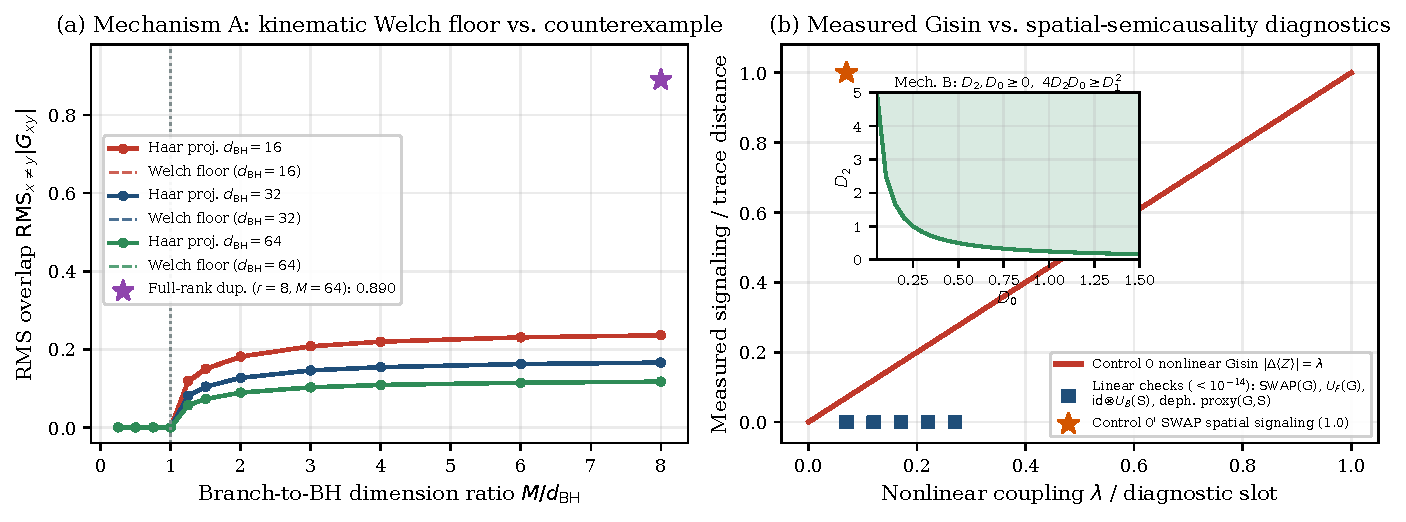
\includegraphics[width=\linewidth]{figures/fig4_branch_coupling_gate.pdf}
  \caption{Suite~G5 (Proposition~\ref{prop:branch-coupling}). (a)~Mechanism~(A): kinematic state-distinguishability RMS off-diagonal Gram overlap $\RMS_{x\neq y}|G_{xy}|$ vs.\ $M/d_{\mathrm{BH}}$ for column-normalized Haar projections ($d_{\mathrm{BH}}\in\{16,32,64\}$) tracking slightly above the Welch lower bound \eqref{eq:welch-floor} ($0.11715\ge 0.11704$ at $d_{\mathrm{BH}}=64, M=512$, reflecting non-tightness after column normalization), alongside the full-rank duplicated-frame counterexample ($r=8,M=64$, purple star: $\RMS=0.88976\gg \mathrm{Welch}=1/3$) confirming that \eqref{eq:welch-floor} is a lower bound only. (b)~Actual measured diagnostics explicitly naming each tested operation: Control~0 nonlinear Gisin bias $|\Delta\langle Z\rangle|=\lambda$ (red), Control~0$'$ $\mathrm{SWAP}$ spatial signaling trace distance $1.0$ (orange star) despite zero Gisin error, and the five zero-level linear checks ($<10^{-14}$, blue squares) for $\mathrm{SWAP}$ (Gisin), Mech.~(A) fundamental unitary $U_F$ (Gisin), local unitary $\id_A\otimes U_B$ (spatial semicausality), and Mech.~(B)'s representative local linear dephasing channel $\Phi_{\mathrm{deph}}(\rho)=0.7\rho+0.3 Z\rho Z$ (Gisin and local semicausality); inset shows Mech.~(B)'s $2\times 2$ PSD region $D_2,D_0\ge 0$, $4D_2 D_0\ge D_1^2$.}
  \label{fig:branch-coupling}
\end{figure}

Table~\ref{tab:gate} and Figure~\ref{fig:branch-coupling} summarize Suite~G5: Control~0 fails Gisin independence ($\Delta\langle Z\rangle=\lambda$); Control~0$'$ ($\mathrm{SWAP}$) proves Gisin independence ($0.0$) does not imply spatial semicausality ($1.0$); Mechanism~(A) separates its non-TP dictionary (trine ETF max output trace $1.5$, raw $\sum|G_{x0}|^2=1.5$, tight-frame POVM error $5.21\times 10^{-16}$; $r=3,M=8$ column-normalized Haar projection confirming non-tightness $\|VV^\dagger-\frac{8}{3}\1_3\|_F=0.57155$ and naive POVM error $0.21433$ vs.\ canonical dual POVM error $1.40\times 10^{-15}$) from linear fundamental evolution ($U_F$ Gisin $0.0$; separate local $\id_A\otimes U_B$ semicausal $1.11\times 10^{-16}$) and exhibits both ETF saturation ($1.67\times 10^{-16}$) and the full-rank duplicated-frame counterexample ($\RMS=0.88976$ vs.\ Welch $1/3$); Mechanism~(B) audits $2\times 2$ real symmetric coefficient-matrix eigenvalues ($+0.09501$ vs.\ $-0.14403$) alongside Gisin ($0.0$) and local-semicausal ($5.55\times 10^{-17}$) residuals on the representative local dephasing proxy $\Phi_{\mathrm{deph}}(\rho)=0.7\rho+0.3 Z\rho Z$ (without claiming a full spacetime CQ gravity generator audit); and Mechanism~(C) separates the modular $\bbZ_4$ toy ($\|C_{\mathrm{tot}}\psi_C\|=\sqrt{12}$, $\|[C_{\mathrm{tot}},O_A^{\mathrm{dr}}]\|_F=4\sqrt{8}$) from the exact $C_{\mathrm{tot}}=0$ bipolar-clock model ($K_{\mathrm{bi}}=5$, $\|C_{\mathrm{tot}}\psi_{\mathrm{exact}}\|=0.0$, $\|[C_{\mathrm{tot}},O_A^{\mathrm{ex}}]\|_F=0.0$, $\|O_A^{\mathrm{ex}}\psi_{\mathrm{exact}}\|=\sqrt{4/5}=0.89443$, entangled $I=2\ln 5=3.21888$ nats vs.\ product $I=0.0$, local constraint-commuting dephasing difference $5.10\times 10^{-17}$ vs.\ global $C_{\mathrm{tot}}$-commuting witness gap $0.40000$) and its completed local CPTP channel $\Phi_A^{\mathrm{ex}}$ (completeness error $0.0$, $[C_{\mathrm{tot}},K_0\otimes\1_B]$ norm $0.0$, $K_1$ success probability $4/5$, conditional $B$-clock trace shift $1/5=0.20000$, non-selective spatial semicausal trace distance $0.0$, and output constraint residual $0.0$).

\begin{table}[!tb]
\centering
\caption{Five-property causal/linear audit separating state positivity, linear CP, TP/TNI, Gisin ensemble independence, and spatial semicausality (Proposition~\ref{prop:branch-coupling}, Suite~G5).}
\label{tab:gate}
\scriptsize
\setlength{\tabcolsep}{3.2pt}
\begin{tabular}{@{} >{\raggedright\arraybackslash}p{2.9cm} c >{\centering\arraybackslash}p{2.0cm} c c >{\raggedright\arraybackslash}p{2.8cm} @{}}
\toprule
Object / Mechanism & State pos./norm & Linear CP & TP / TNI & Gisin indep. & Spatial semicausal \\
\midrule
Control~0: nonlinear $\Phi_\lambda$ & Pass & \textbf{FAIL} & Unit Tr only & \textbf{FAIL} ($\lambda$) & \textbf{FAIL} (TD $=\lambda/2$ per-branch on EPR) \\
Control~0$'$: $\mathrm{SWAP}$ gate & Pass & Pass & Pass (unitary) & Pass ($0.0$) & \textbf{FAIL} (TD $=1.0$) \\
Mech.~(A) dict.\ $\mathcal{V}(\rho)=V\rho V^\dagger$ & Pos.\ only & Pass & \textbf{FAIL} ($\mathrm{Tr}=1.5$) & Linear map & N/A (code dictionary) \\
Mech.~(A) fund.\ ($U_F$; $\id_A\!\otimes\!U_B$) & Pass & Pass & Pass & Pass ($U_F$; $0.0$) & Pass ($\id_A\!\otimes\!U_B$; $<10^{-15}$) \\
Mech.~(B): CQ $2\times 2$ / deph.\ proxy & Pass & $D_2,D_0\ge 0$, $4D_2D_0\ge D_1^2$ & Pass (proxy) & Pass (proxy; $0.0$) & Pass (local deph.\ proxy) \\
Mech.~(C.2): local CPTP $\Phi_A^{\mathrm{ex}}$ & Pass & Pass & Pass ($K_0,K_1$) & Pass ($0.0$) & Pass (local; $0.0$) \\
\bottomrule
\end{tabular}
\end{table}

%==============================================================================
\section{Formal Verification, Numerical Audit, and Explicit Trust Boundary}\label{sec:verification}
%==============================================================================

To keep machine-checked proofs, analytical finite-dimensional and continuum arguments, and numerical evidence strictly separated, Table~\ref{tab:trust-boundary} summarizes the trust boundary of the independent Lean~4.36.0 + Mathlib4 library \code{OSTQD\_Layer2} (\textbf{61 audited theorem declarations}, standard three axioms \code{propext}, \code{Classical.choice}, \code{Quot.sound} only, zero forbidden tokens, zero tactic/linter warnings---distinct from Lean~4.36.0's benign \code{module}-system import notice; complete log archived in \code{lean4/VERIFICATION\_LOG.txt}; full one-to-one declaration inventory in Appendix~\ref{app:lean-inventory}) alongside the deterministic Python verification suite G1--G5 (\textbf{329 recorded scientific numeric fields}, seed \code{20261128}, in \code{docs/numerical\_verification.json}). As in \cite{Soga2026OSTQD,Soga2026OSTQDSK}, declaration and numeric field counts measure audit coverage rather than physical novelty.

\begin{table}[!tb]
\centering
\caption{Summary trust boundary separating Lean~4.36.0 machine-checked finite-dimensional cores (\code{OSTQD\_Layer2}, 61 audited theorem declarations; full list in Appendix~\ref{app:lean-inventory}) from analytical steps outside Lean and numerical audits G1--G5.}
\label{tab:trust-boundary}
\scriptsize
\begin{tabular}{@{} >{\raggedright\arraybackslash}p{2.3cm} >{\raggedright\arraybackslash}p{6.2cm} >{\raggedright\arraybackslash}p{6.2cm} @{}}
\toprule
Manuscript result & Machine-checked Lean~4.36.0 core (61 audited theorems) & Analytical / numerical / physical steps outside Lean \\
\midrule
Core instruments (\S\ref{sec:framework}) &
\code{Basic.lean} (6): Frobenius vanishing/trace identities, Kraus trace preservation, POVM Born-weight sum and convex affineness. &
Infinite-dimensional normal CP instrument predual duality; operational modeling with local probe QFTs \cite{FewsterVerch2020}. \\
\midrule
Theorem~\ref{thm:steering} (\S\ref{sec:steering}) &
\code{Theorem1\_SteeringNoGo.lean} (10): Schmidt assemblage identity, zero-steering triviality, Frobenius floor, product/classical/two-qubit isotropic controls, rational $S=14/5$ CHSH, $\mathrm{Bool}^4$ Farkas impossibility, FR $1/12$ witness. &
Singular-value inequality $\|\cdot\|_1\ge\|\cdot\|_F$ and general finite-dimensional floor $s_{\min}(T_\rho|_{\mathsf{H}_0})$ (proved analytically; G1 audits Schmidt, isotropic, and kernel-carrying controls); spacetime extended Wigner's friend protocols and operational AOE identification \cite{Bong2020,HausmannRenner2025}. \\
\midrule
Theorem~\ref{thm:branching} (\S\ref{sec:branching}) &
\code{Theorem2\_BranchingModels.lean} (14): CHSH negativity floor $(S-2)/4$, rational $1/5$ witness, barycenter/commuting marginals, equal-marginal \& Kraus-flip counterexamples, 4D Wigner's friend CNOT dilation \& premeasurement-isometry $J$ Kraus orthogonality vs.\ unrestricted $|01\rangle$, unique matrix trace representation \& complete positive linear-functional POVM theorem, replacer non-uniqueness, non-affine control, exact Kraus record-agreement equivalence \eqref{eq:kraus-record-orthog}, minimal two-path diamond. &
Positive-cone extension from density states to $\bbC$-linear functionals on $M_d(\bbC)$ (analytical); LP visibility sweep (G2); infinite-dimensional $L^1(\cM,\tau)^*\cong\cM$ trace duality; categorical relativistic presheaves and general sheaf cohomology \cite{AbramskyBrandenburger2011}. \\
\midrule
Theorem~\ref{thm:type2-clock} \& Cor.~\ref{cor:grav-entropy} (\S\ref{sec:type2}) &
\code{Theorem3\_ClockTypeII.lean} (8): finite $\bbZ_K$ Umegaki conditional expectation (5 axioms), covariant Born invariance, additive Segal-entropy shift cancellation (algebraic scalar identity), scalar regularized logarithm domination bounds. &
Type~$\mathrm{III}_1\to\mathrm{II}_\infty/\mathrm{II}_1$ modular crossed products and finite-trace corners \cite{Takesaki1973,Witten2022,JensenSorceSperanza2023}; unbounded regularized positive-pairing finite-entropy proof and Araki monotonicity \cite{Araki1977}; conditional semiclassical $S_\tau=S_{\mathrm{gen}}+C+\delta(\rho)$ identity (Cor.~\ref{cor:grav-entropy}, G3). \\
\midrule
Theorem~\ref{thm:nonisometric} (\S\ref{sec:nonisometric}) &
\code{Theorem4\_NonIsometricPullback.lean} (10): pullback POVM sum, cyclic Born identity, kernel annihilation, singular-value bound, renormalized $\ell^1$ triangle inequality, real scalar polar bounds \eqref{eq:polar-sharp-unnorm}--\eqref{eq:polar-sharp-norm} + saturation, general sequential compatibility \eqref{eq:seq-compat}, compatible $N_{\mathrm{BH},0}=2$ kernel witness, normalized-filter Gisin bias witness. &
Matrix polar decomposition $VP_\cC=WM$, purification contraction to mixed states, Helstrom POVM variational identity; Stinespring converse \cite{Watrous2018}; Haar concentration \cite{Akers2024}; sequential $W_n^{\mathrm{seq}}$ vs.\ postselected $(V_n,W_{\mathrm{pol},n})$ and conditioned $\tilde{V}_n$ audits \cite{Chiribella2009,DeWolfeHigginbotham2023} (G4); autonomous gravity Hamiltonian. \\
\midrule
Proposition~\ref{prop:branch-coupling} (\S\ref{sec:branch-coupling}) &
\code{Proposition5\_BranchCoupling.lean} (13): Gisin nonlinear wall, general local semicausality, SWAP spatial-signaling counterexample, complex Welch bound \& crosstalk floor, trine non-TP/POVM witness, general full-rank duplicated-frame counterexample, CQ $2\times 2$ PSD, dressed commutativity, arbitrary-$m$ exact $C_{\mathrm{tot}}=0$ bipolar clocks, finite-matrix CPTP completion \eqref{eq:bipolar-cptp}, local constraint-commuting dephasing invariance. &
Column-normalized Haar projections \& canonical dual POVM audit and clock mutual information $I(C_A:C_B)$ (G5); dynamical gravitational transition rates (not implied by kinematic Welch overlap); full relativistic CQ gravity master generators \cite{Oppenheim2023PRX} and experimental collapse bounds \cite{Donadi2021}. \\
\bottomrule
\end{tabular}
\end{table}

\subsection{Finite-Dimensional Analytical Bridges and Missing Mathlib4 v4.36.0 Continuum Libraries}\label{sec:mathlib-gaps}

Every finite-dimensional algebraic statement listed in the middle column of Table~\ref{tab:trust-boundary} is machine-checked in \code{OSTQD\_Layer2} without custom \code{axiom} declarations, strictly at the proposition granularity stated there (for example, \code{segal\_\allowbreak entropy\_\allowbreak scale\_\allowbreak invariance} checks additive shift cancellation while unbounded density trace formulas are proved analytically; \code{sharp\_\allowbreak polar\_\allowbreak *\_\allowbreak pure\_\allowbreak bound} checks the real scalar inequalities and equality witnesses while matrix polar decomposition, purification contraction, and Helstrom optimization connect them to \eqref{eq:polar-sharp-unnorm}--\eqref{eq:polar-sharp-norm}; and \code{exact\_\allowbreak bipolar\_\allowbreak clock\_\allowbreak cptp\_\allowbreak channel\_\allowbreak completion} checks finite-matrix Kraus completeness and $C_{\mathrm{tot}}$-commutativity, which combines with \code{local\_\allowbreak channel\_\allowbreak spatial\_\allowbreak semicausality} to yield spatial semicausality). For transparency, the steps proved analytically (or audited numerically) outside Lean~4.36.0 fall into two distinct groups:

First, four \emph{finite-dimensional analytical bridges} are intentionally proved on paper and checked numerically rather than formalized inside Lean: (a)~extending positive affine functionals defined only on density states to $\bbC$-linear functionals on $M_d(\bbC)$ in Theorem~\ref{thm:branching}(c) (once $\bbC$-linear, trace representation, Hermiticity, PSD, completeness, and $E_x\le\1$ are machine-checked in \code{finite\_dim\_complete\_positive\_functional\_povm\_rep}); (b)~the singular-value norm inequality $\|\cdot\|_1\ge\|\cdot\|_F$ and general singular-value floor $s_{\min}(T_\rho|_{\mathsf{H}_0})$ in Theorem~\ref{thm:steering}(b); (c)~matrix polar decomposition, purification partial-trace contraction from pure to mixed states, and the Helstrom POVM variational identity in Theorem~\ref{thm:nonisometric}(b); and (d)~direct evaluation of von Neumann entropy / clock mutual information $I(C_A:C_B)=2\ln(2m+1)$ in Proposition~\ref{prop:branch-coupling}(C.2).

Second, six \emph{infinite-dimensional operator-algebraic and probabilistic domains} remain outside Lean~4.36.0 because the prerequisite libraries are not yet present in Mathlib4 (\code{v4.36.0}):
\begin{enumerate}
  \item \emph{von Neumann algebra type classification and semifinite factor theory:} Mathlib4 provides basic $C^*$-algebra and bounded-operator infrastructure, but lacks Murray--von Neumann / Connes classification of Types~$\mathrm{I}, \mathrm{II}_1, \mathrm{II}_\infty, \mathrm{III}_1$ and faithful normal semifinite weights/traces.
  \item \emph{Noncommutative $L^1(\cM,\tau)$ predual spaces and semifinite Segal trace integration:} required to formalize the infinite-dimensional trace-duality isomorphism $L^1(\cM,\tau)^*\cong\cM$ (Theorem~\ref{thm:branching}(c) continuum lift) and normal CP instrument duality.
  \item \emph{Unbounded self-adjoint spectral measures and Borel functional calculus for $\rho\ln\rho$:} required to formalize the finite-entropy domain $\cD_{\mathrm{ent}}(\cM,\tau)$ and operator-monotone regularization $\ln(\bar{\rho}_O+\eta\1)$ in Theorem~\ref{thm:type2-clock}(b).
  \item \emph{Tomita--Takesaki modular theory and Takesaki crossed-product duality:} modular operators $\Delta_\omega$, modular conjugations $J_\omega$, modular automorphism groups $\sigma^\omega_t$, and the Type~$\mathrm{II}_\infty$ continuous core $\cM\rtimes_{\sigma^\omega}\bbR$ with finite-trace corners $0<\tau(P)<\infty$ (Corollary~\ref{cor:grav-entropy}).
  \item \emph{Araki relative modular operators $\Delta_{\omega,\phi}$ and operator-algebraic relative entropy monotonicity:} required to formalize $0\le D(\rho_{O|x}\|\bar{\rho}_O)\le -\ln p_x$ directly on general semifinite factors.
  \item \emph{Non-asymptotic Haar / L\'evy measure concentration on unitary groups $U(d)$:} required to formalize probabilistic approximate-isometry bounds \cite{Akers2024} beyond the exact expectation identity $\mathbb{E}[\tilde{V}_n^\dagger\tilde{V}_n]=\1_C$.
\end{enumerate}
Explicitly isolating both finite-dimensional bridges and continuum library gaps avoids axiomatic shortcuts while keeping the machine-checked kernel auditable on standard axioms alone.

%==============================================================================
\section{Discussion and Open Frontiers}\label{sec:conclusion}
%==============================================================================

Continuing \cite{Soga2026OSTQD,Soga2026OSTQDSK}, this study has established a conditional, formally and numerically audited algebraic map of Layer~2 selective instruments, semifinite Segal-entropy branch splitting, sharp non-isometric pullback bounds, and inter-branch coupling gates:
\begin{itemize}
  \item \textbf{Established results within stated hypotheses:}
  (i)~In finite dimensions, on any bipartite state whose centered assemblage map $T_\rho$ is injective on $\mathsf{H}_0=\{H=H^\dagger:\Tr(\rho_R H)=0\}$ (including every full-Schmidt-rank pure state and every separable or entangled two-qubit isotropic state $0<v<1$), forbidding single-setting outcome-conditioned remote state change forces label-trivial POVMs $E_x=p_x\1_R$ (with converse construction $E_\pm=\frac{1}{2}\1_R\pm tH$ whenever $\ker T_\rho|_{\mathsf{H}_0}\neq\{0\}$ and quantitative floors $\lambda_{\min}$, $v/2$, and $s_{\min}(T_\rho|_{\mathsf{H}_0})$), while the rational witness $S=14/5$ certifies two-setting Local Friendliness and $\mathrm{Bool}^4$ global-section obstructions (Theorem~\ref{thm:steering});
  (ii)~Global-coupling single-realization models (Model~I) incur sharp signed negativity $\cN_{\min}=\max\{0,(S_*-2)/4\}$ over all eight CHSH facet orientations (i.e.\ $(S-2)/4$ for a violating facet $S>2$, equivalent to \cite{Oas2014}, saturated at $1/5$ for $S=14/5$), whereas context-indexed Born-weighted branch measures (Model~II) drop single-space (ZSC), preserve ensemble linearity, characterize all-input sequential record agreement via \eqref{eq:kraus-record-orthog}, separate all-logical-input record-preserving CPL ($P(x_S\neq x_F)=0$ via premeasurement isometry $J$) from record-erasing interference ($1$ vs.\ $1/2$) and two-path record-subalgebra agreement in finite-dimensional dilations, and admit unique POVM representation on any semifinite algebra via $L^1(\cA_O,\tau_O)^*\cong\cA_O$ without fixing Layer~1 unravelings (Theorem~\ref{thm:branching});
  (iii)~Separating a finite $\bbZ_K$ toy analogue from the continuum setting, a non-circular regularized positive-pairing proof on any semifinite von Neumann algebra $(\cM,\tau)$ yields the trace-scale-invariant Segal-entropy branch split $\Delta S_\tau^{\mathrm{L1}}-\overline{\Delta S}_\tau^{\mathrm{L2}}=\chi_\tau\in[0,H(\{p_x\})]$ (with a gravity-free Type~$\mathrm{II}_1$ saturation witness and Ozawa's negative-gain control, Theorem~\ref{thm:type2-clock}), while Corollary~\ref{cor:grav-entropy} isolates the conditional semiclassical identity governing $S_{\mathrm{gen}}$ up to clock/ADM and clock--field corrections $\delta(\rho)$;
  (iv)~In finite dimensions, uniformly sharp polar-isometric $\ell^1$ bounds $\sqrt{1+\varepsilon}-\sqrt{1-\varepsilon}$ and $2\varepsilon/(1+\sqrt{1-\varepsilon^2})$ (embedding \cite{Kantorovich1948,Gustafson1968} with mixed-state purification contraction, Helstrom-POVM saturation, and contractive Kraus reweighting vs.\ Gisin bias $\varepsilon/2$) quantify Born-weight pullback defects whenever $\varepsilon<1$, while a strictly causal sequential unitary evaporation circuit $W_n^{\mathrm{seq}}$ obeying \eqref{eq:seq-compat} identically is explicitly separated from general co-isometric postselected dictionaries $(V_n,W_{\mathrm{pol},n})$ (with Stinespring equivalence \cite{Watrous2018}, a compatible kernel-carrying witness, fixed-seed incompatibility on both $W_{\mathrm{pol},n}$ and success-conditioned $\tilde{V}_n$ \cite{Chiribella2009}, and contrast against dynamical backwards-forwards circuit dictionaries \cite{DeWolfeHigginbotham2023}, Theorem~\ref{thm:nonisometric}); and
  (v)~A five-property audit separates Gisin ensemble independence, spatial semicausality, dictionary non-TP defects, kinematic Welch distinguishability lower bounds, and an exact $C_{\mathrm{tot}}=0$ bipolar-clock local CPTP channel completion $\Phi_A^{\mathrm{ex}}$ (showing also local constraint-commuting dephasing invariance and conditional $1/K_{\mathrm{bi}}$ vs.\ non-selective $0$ $B$-clock updating) vs.\ modular $\bbZ_K$ toys (Proposition~\ref{prop:branch-coupling}).
  \item \textbf{Concrete open frontiers:}
  (1)~\emph{Categorical relativistic Model~II gluing:} promoting the finite-dimensional Wigner's friend dilation and two-path diamond of Theorem~\ref{thm:branching}(b) to a covariant category of Fewster--Verch local probe QFTs \cite{FewsterVerch2020} with path-independent record-transfer channels across general curved-spacetime observer posets;
  (2)~\emph{Gravitational semiclassical control of $\delta(\rho)$:} constructing concrete gravitational crossed-product instruments preserving a Type~$\mathrm{II}_1/\mathrm{II}_\infty$ corner and certifying uniform semiclassical bounds $|\delta(\rho)|\le\eta_{\mathrm{sc}}$ across branches in Corollary~\ref{cor:grav-entropy};
  (3)~\emph{Microscopic autonomous $U(N)$ gauge-matrix dynamics and Gauss-law port closure:} testing whether a single time-independent $U(N)$ matrix Hamiltonian with block decomposition $N=N_A+N_B$ and off-diagonal open-string modes $(X^I_{AB},\Psi^\alpha_{AB})$ dynamically generates emergent $(t,s)$ open dynamics, an autonomous sequential Page curve obeying \eqref{eq:seq-compat}, complexity-protected non-isometric interior maps, and spin-blind inward port closure (or a sharp Gauss-law obstruction) \cite{BFSS1997,IKKT1997}; and
  (4)~\emph{Non-perturbative UV matrix completion:} investigating whether a background-independent BFSS/IKKT-type matrix action can simultaneously reproduce low-energy SK/JT thermodynamic audits \cite{Soga2026OSTQDSK}, continuum Type~$\mathrm{II}_1/\mathrm{II}_\infty$ observer-clock algebras, and dynamical non-isometric horizon encodings beyond the semiclassical regime.
\end{itemize}

%==============================================================================
\appendix
\section{Complete One-to-One Inventory of Audited Lean~4.36.0 Declarations}\label{app:lean-inventory}
%==============================================================================

For independent kernel auditing against \code{lean4/OSTQD\_Layer2/AxiomCheck.lean} and \code{lean4/VERIFICATION\_LOG.txt}, all 61 audited theorem declarations in \code{OSTQD\_Layer2} (each verified to depend strictly on \code{[propext, Classical.choice, Quot.sound]}) are listed below by module:
{\raggedright
\begin{itemize}
  \item \code{Basic.lean} (6): \code{frobNormSq\_\allowbreak eq\_\allowbreak zero\_\allowbreak iff}, \code{trace\_\allowbreak conjTranspose\_\allowbreak mul\_\allowbreak self\_\allowbreak re}, \code{trace\_\allowbreak mul\_\allowbreak conjTranspose\_\allowbreak self\_\allowbreak re}, \code{nonSelectiveMap\_\allowbreak trace\_\allowbreak preserving}, \code{bornWeight\_\allowbreak sum\_\allowbreak eq\_\allowbreak trace}, \code{bornWeight\_\allowbreak convex\_\allowbreak affine}.
  \item \code{Theorem1\_\allowbreak SteeringNoGo.lean} (10): \code{partialTraceR\_\allowbreak schmidt\_\allowbreak eq\_\allowbreak assemblage}, \code{schmidt\_\allowbreak nonselective\_\allowbreak no\_\allowbreak signaling}, \code{zero\_\allowbreak steering\_\allowbreak iff\_\allowbreak trivial\_\allowbreak effect}, \code{steering\_\allowbreak frobenius\_\allowbreak lower\_\allowbreak bound}, \code{product\_\allowbreak state\_\allowbreak zero\_\allowbreak steering\_\allowbreak control}, \code{classical\_\allowbreak correlated\_\allowbreak x\_\allowbreak basis\_\allowbreak zero\_\allowbreak steering\_\allowbreak control}, \code{rational\_\allowbreak lf\_\allowbreak observables\_\allowbreak involutive\_\allowbreak and\_\allowbreak chsh}, \code{rational\_\allowbreak lf\_\allowbreak no\_\allowbreak nonnegative\_\allowbreak global\_\allowbreak section}, \code{frauchiger\_\allowbreak renner\_\allowbreak contradiction\_\allowbreak witness}, \code{werner\_\allowbreak mixed\_\allowbreak state\_\allowbreak zero\_\allowbreak steering\_\allowbreak iff\_\allowbreak trivial}.
  \item \code{Theorem2\_\allowbreak BranchingModels.lean} (14): \code{signed\_\allowbreak global\_\allowbreak section\_\allowbreak negativity\_\allowbreak lower\_\allowbreak bound}, \code{signed\_\allowbreak global\_\allowbreak section\_\allowbreak rational\_\allowbreak witness\_\allowbreak sharp}, \code{presheaf\_\allowbreak barycenter\_\allowbreak reproduces\_\allowbreak layer1}, \code{commuting\_\allowbreak records\_\allowbreak cpl\_\allowbreak marginals}, \code{nonaffine\_\allowbreak quadratic\_\allowbreak weight\_\allowbreak fails\_\allowbreak convexity}, \code{equal\_\allowbreak marginals\_\allowbreak do\_\allowbreak not\_\allowbreak imply\_\allowbreak record\_\allowbreak agreement}, \code{commuting\_\allowbreak effects\_\allowbreak kraus\_\allowbreak flip\_\allowbreak counterexample}, \code{wigner\_\allowbreak friend\_\allowbreak record\_\allowbreak preserving\_\allowbreak vs\_\allowbreak interference}, \code{finite\_\allowbreak dim\_\allowbreak linear\_\allowbreak functional\_\allowbreak unique\_\allowbreak povm\_\allowbreak rep}, \code{finite\_\allowbreak dim\_\allowbreak complete\_\allowbreak positive\_\allowbreak functional\_\allowbreak povm\_\allowbreak rep}, \code{replacer\_\allowbreak unraveling\_\allowbreak weight\_\allowbreak nonuniqueness}, \code{sequential\_\allowbreak record\_\allowbreak agreement\_\allowbreak iff\_\allowbreak kraus\_\allowbreak orthogonality}, \code{two\_\allowbreak path\_\allowbreak diamond\_\allowbreak record\_\allowbreak subalgebra\_\allowbreak agreement}, \code{wigner\_\allowbreak friend\_\allowbreak premeasurement\_\allowbreak kraus\_\allowbreak orthogonality}.
  \item \code{Theorem3\_\allowbreak ClockTypeII.lean} (8): \code{condExp\_\allowbreak invariant}, \code{condExp\_\allowbreak unital}, \code{condExp\_\allowbreak trace\_\allowbreak preserving}, \code{condExp\_\allowbreak bimodule}, \code{condExp\_\allowbreak idempotent}, \code{covariant\_\allowbreak effect\_\allowbreak born\_\allowbreak invariance}, \code{segal\_\allowbreak entropy\_\allowbreak scale\_\allowbreak invariance}, \code{regularized\_\allowbreak log\_\allowbreak domination\_\allowbreak bounds}.
  \item \code{Theorem4\_\allowbreak NonIsometricPullback.lean} (10): \code{pullback\_\allowbreak povm\_\allowbreak sum}, \code{pullback\_\allowbreak born\_\allowbreak cyclic\_\allowbreak identity}, \code{kernel\_\allowbreak vector\_\allowbreak total\_\allowbreak annihilation}, \code{polar\_\allowbreak singular\_\allowbreak value\_\allowbreak bound}, \code{renormalized\_\allowbreak tv\_\allowbreak defect\_\allowbreak bound}, \code{sharp\_\allowbreak polar\_\allowbreak unnormalized\_\allowbreak pure\_\allowbreak bound}, \code{sharp\_\allowbreak polar\_\allowbreak normalized\_\allowbreak pure\_\allowbreak bound}, \code{sequential\_\allowbreak evaporation\_\allowbreak radiation\_\allowbreak compatibility}, \code{nonisometric\_\allowbreak kernel\_\allowbreak compatible\_\allowbreak two\_\allowbreak step\_\allowbreak witness}, \code{postselected\_\allowbreak normalized\_\allowbreak gisin\_\allowbreak bias\_\allowbreak witness}.
  \item \code{Proposition5\_\allowbreak BranchCoupling.lean} (13; corresponding to Proposition~\ref{prop:branch-coupling}): \code{gisin\_\allowbreak nonlinear\_\allowbreak map\_\allowbreak trace\_\allowbreak preserving}, \code{gisin\_\allowbreak epr\_\allowbreak signaling\_\allowbreak bias}, \code{welch\_\allowbreak gram\_\allowbreak general\_\allowbreak bound}, \code{welch\_\allowbreak rank\_\allowbreak forced\_\allowbreak branch\_\allowbreak crosstalk}, \code{oppenheim\_\allowbreak cq\_\allowbreak psd\_\allowbreak tradeoff}, \code{two\_\allowbreak clock\_\allowbreak dressed\_\allowbreak commutativity}, \code{local\_\allowbreak channel\_\allowbreak spatial\_\allowbreak semicausality}, \code{swap\_\allowbreak gate\_\allowbreak ensemble\_\allowbreak independent\_\allowbreak yet\_\allowbreak signaling}, \code{trine\_\allowbreak frame\_\allowbreak exceeds\_\allowbreak unit\_\allowbreak trace\_\allowbreak and\_\allowbreak povm\_\allowbreak norm}, \code{full\_\allowbreak rank\_\allowbreak duplicated\_\allowbreak frame\_\allowbreak exceeds\_\allowbreak welch\_\allowbreak lower\_\allowbreak bound}, \code{exact\_\allowbreak bipolar\_\allowbreak clock\_\allowbreak constraint\_\allowbreak entangled\_\allowbreak and\_\allowbreak product}, \code{exact\_\allowbreak bipolar\_\allowbreak clock\_\allowbreak cptp\_\allowbreak channel\_\allowbreak completion}, \code{bipolar\_\allowbreak clock\_\allowbreak local\_\allowbreak constraint\_\allowbreak commuting\_\allowbreak dephasing\_\allowbreak invariance}.
\end{itemize}
}

%==============================================================================
\section*{Author Contributions and AI Disclosure}\label{sec:ai-disclosure}
%==============================================================================
\addcontentsline{toc}{section}{Author Contributions and AI Disclosure}

Following transparent AI disclosure practices in theoretical high-energy physics \cite{Michel2026}, human and AI contributions are explicitly separated:
\begin{itemize}
  \item \textbf{Human author (Yohtaro Soga):} Conceived the overarching research program linking black hole evaporation observer discrepancies to observer-separated two-time dynamics, Layer~2 selective instruments, Born-weighted branching, and inter-branch gravitational coupling; defined the scope separation, epistemic standards, active branch-coupling audit criteria, and falsification criteria; and directed all theoretical and architectural decisions.
  \item \textbf{AI research assistant (Google Antigravity / Gemini):} Conducted the primary literature audit across quantum steering, signed-probability negativity, sheaf-theoretic contextuality, Local Friendliness / Wigner's friend, causal quantum operations, semifinite Segal--Holevo entropy, Type~II crossed products, Kantorovich--Gustafson operator-angle bounds, non-isometric codes, Welch bounds, and classical--quantum gravity; formulated and proved Theorems~\ref{thm:steering}--\ref{thm:nonisometric}, Corollary~\ref{cor:grav-entropy}, and Proposition~\ref{prop:branch-coupling}; implemented and executed the deterministic G1--G5 Python verification and figure-generation suite; authored and kernel-verified all 61 audited Lean~4.36.0 / Mathlib4 declarations in \code{OSTQD\_Layer2}; and assisted with LaTeX manuscript drafting and compilation.
\end{itemize}
All 61 audited Lean~4.36.0 theorem declarations are machine-checked in \code{lean4/\allowbreak VERIFICATION\_\allowbreak LOG.txt}, and all 329 recorded scientific numeric fields (G1--G5) and four vector PDF figures are independently reproducible from \code{scripts/\allowbreak verify\_\allowbreak paper3\_\allowbreak layer2\_\allowbreak type2.py}.

\bibliographystyle{unsrt}
\bibliography{references}

\end{document}
